% template.tex, dated April 5 2013
% This is a template file for Annual Reviews 1 column Journals
%
% Compilation using ar-1col.cls' - version 1.0, Aptara Inc.
% (c) 2013 AR
%
% Steps to compile: latex latex latex
%
% For tracking purposes => this is v1.0 - Apr. 2013

\documentclass[letterpaper]{ar-1col}
% \documentclass[letterpaper,draft]{ar-1col}
\usepackage[numbers]{natbib}
\usepackage[left=35mm,top=26mm,right=26mm,bottom=15mm]{geometry}




\usepackage[american]{babel}
% \usepackage{amsmath}
\usepackage[version=3]{mhchem} 
% % \usepackage{fixltx2e}
% % \usepackage{refcount}
\usepackage{siunitx}
% % \usepackage{lastpage}
% % \usepackage{textcomp}
% \usepackage{mathtools}
% 
% \usepackage{xfrac}
\usepackage{lmodern}
\usepackage[hidelinks]{hyperref}
% % \usepackage{cool}
% % \usepackage{cancel}
% \usepackage{microtype}
% \usepackage{listings}
% % \usepackage{mcode}
\usepackage [autostyle, english = american]{csquotes}
% % \usepackage{longtable}
% % \usepackage{subcaption}
% \usepackage{booktabs,siunitx}
% \usepackage{gensymb}
% \usepackage[normalem]{ulem}

% \usepackage{mathtools, cuted}
\usepackage{wrapfig}


% \usepackage[usenames,dvipsnames,svgnames,table]{xcolor}
% \usepackage{color}

% \usepackage[colorinlistoftodos]{todonotes}

% \usepackage[section]{placeins}
% \usepackage{multirow}

% \usepackage{lineno}

\usepackage{graphicx}% Include figure files
% \usepackage{dcolumn}% Align table columns on decimal point



% Sin and Cos with auto-parentheses 
\newcommand{\sinp}[1]{\sin{\left( #1\right)}}
\newcommand{\cosp}[1]{\cos{\left( #1\right)}}
\newcommand{\expp}[1]{\exp{\left( #1\right)}}
\newcommand{\sinhp}[1]{\sinh{\left( #1\right)}}
\newcommand{\lnp}[1]{\ln{\left( #1\right)}}
\newcommand{\pp}[1]{\left( #1\right)}
\newcommand{\sci}[2]{ #1 \cdot 10^{#2}\ }
\newcommand{\angstrom}{\mbox{\normalfont\AA}}
\newcommand{\norm}[1]{\lVert #1 \rVert}

\newcommand{\textred}[1]{\textcolor{red}{ #1}}
\newcommand{\redactedit}[1]{\textcolor{blue}{ \sout{#1}}}

\newcommand{\cmmnt}[1]{}


\newcommand{\colornote}[1]{\textcolor{red}{ COMMENT\large\footnote{\textcolor{red}{#1}}}}

\newcommand{\comment}[1]{\todo[color=blue!20!white,inline]{ASV: #1}} 

\newcommand{\etal}{\emph{et\,al.}} 


% Tweak sim for better inline text tilde
\newcommand{\mytilde}{\raisebox{0.5ex}{\texttildelow}}
% \newcommand{\mytilde}{\raise.17ex\hbox{$\scriptstyle‌​\sim$}}

% \sisetup{separate-uncertainty=true,table-space-text-post = *}

\newcommand{\minitab}[2][l]{\begin{tabular}{#1}#2\end{tabular}}

% \newcounter{subfigure}[figure]

\newcommand{\subfigimg}[4][,]{%
  \setbox1=\hbox{\noindent\includegraphics[#1]{#3}}% Store image in box
  \leavevmode\rlap{\usebox1}% Print image
  \rlap{\hspace*{#4pt}\raisebox{\dimexpr\ht1-2\baselineskip}{#2}}% Print label
  \phantom{\usebox1}% Insert appropriate spcing
}
% \subfigimg[scale=0.59]{a)}{./figures/after_minimization_plot_alt.pdf}{80pt}

% \usepackage[style=base]{caption}
% \usepackage{subfig}
% Remove a), b), etc labels from subfigs
% \captionsetup[subfigure]{labelformat=empty}
% \captionsetup{style=base} 

% Sick of fighting siunitx - consistent text micro symbol
% DO NOT uncomment this!!! or else broken unicode (Âţ)
% \sisetup{math-micro=\text{µ},text-micro=µ}
% \si\micro
\newcommand{\mmicro}{\si\micro} 

% \usepackage{adjustbox}


% \makeatletter
% % Make common definition of mean
% \newcommand*\mean[1]{\overline{#1\raisebox{3mm}{}}}
% 
% \makeatother

\hyphenation{gamma-rays}
\hyphenation{Spec-tro-met-ers}


% \setcounter{secnumdepth}{4}

% Remove overfull hbox warnings in bibliography
\usepackage{etoolbox}
\apptocmd{\sloppy}{\vbadness 10000\relax}{}{}
% \emergencystretch=1em

\pdfminorversion=7



% 
% 
% 
% Journal template info
% 
% 
% 
% 
% 
% 
% 
% 



% Metadata Information
\jname{Xxxx. Xxx. Xxx. Xxx.}
\jvol{AA}
\jyear{YYYY}
\doi{10.1146/((please add article doi))}


% \makeatletter
%  \def\@textbottom{\vskip \z@ \@plus 1pt}
%  \let\@texttop\relax
% \makeatother


% Document starts
\begin{document}

% Page header
\markboth{Bernstein et al.}{Our Future Nuclear Data Needs}

% Title
\title{Our Future Nuclear Data Needs}


%Authors, affiliations address.
\author{Lee A. Bernstein$^{1,2}$, David A. Brown$^3$, \\Arjan J. Koning$^4$, Brad T. Rearden$^5$,  \\Catherine E. Romano$^6$, Alejandro A. Sonzogni$^3$, Andrew S. Voyles$^{1,2}$, and Walid  Younes$^7$
\affil{$^1$Nuclear Science Division, Lawrence Berkeley National Laboratory,  Berkeley, CA 94720, USA; email: labernstein@lbl.gov}
\affil{$^2$Department of Nuclear Engineering, University of California, Berkeley,  Berkeley, CA 94720, USA}
\affil{$^3$National Nuclear Data Center, Brookhaven National Laboratory, Upton, NY 11973, USA}
\affil{$^4$Arjan's affiliations\textred{Arjan - please provide!}}
\affil{$^5$Brad's affiliations\textred{Brad - please provide!}, Oak Ridge National Laboratory, Oak Ridge, TN 37830, USA}
\affil{$^6$Reactor and Nuclear Systems Division, Oak Ridge National Laboratory, Oak Ridge, TN 37830, USA}
\affil{$^7$\textred{Add Walid's division here}, Lawrence Livermore National Laboratory,  Livermore, CA 94550, USA}}

%Abstract
\begin{abstract}
A well-established knowledge of nuclear phenomena including fission, reaction cross sections, and structure/decay properties, is critical for applications ranging from the design of new reactors, to non-proliferation, to the production of radioisotopes for the diagnosis and treatment of illness.  However, the lack of a well-quantified, predictive theoretical capability means that most nuclear observables must be measured directly in order to \enquote{calibrate} empirical models, which, in turn, provide the data needed for these applications.  In many cases there is either a lack of the data needed to guide the models, or the results of the different measurements are discrepant.  This has led to the development of evaluation methodologies to provide recommended values and uncertainties.  In this article we present the nuclear data evaluation process and the international community that carries it out.  We then discuss new measurements and improved theory and/or modeling needed to address future challenges in applied nuclear science. 
\end{abstract}

%Keywords, etc.
\begin{keywords}
nuclear data,  structure,  reactions, evaluation, fission, medical Isotopes, nuclear energy, nonproliferation, inelastic scattering, level density, radiative strength, $\beta$-decay, reactor antineutrinos
\end{keywords}
\maketitle

%Table of Contents
\tableofcontents


% Heading 1
\section{INTRODUCTION}

\subsection{The Two Faces of Nuclear Data}


Low-energy nuclear science (LENS) \enquote{straddles the fence} between curiosity- and application-driven pursuits.  On the curiosity-driven side, low-energy ($E_x <$ 1--4 MeV) nuclear structure offers a unique laboratory to examine the interplay between single-particle and collective behavior and to explore the transition from quantum to continuum behavior in a mesoscopic setting. LENS also plays an important role in nuclear astrophysics, improving models of stellar energy generation and allowing isotopic abundances to be used to inform models of the astrophysical environments where heavy nuclei are formed.  On the applied side, a well-quantified knowledge of low-lying nuclear structure and reactions is needed to model energy generation and isotope production for medical and industrial uses and for the national security and counter-proliferation communities.   

One hallmark of LENS is that most theoretical descriptions are descriptive rather than rigorously predictive at the level of accuracy and over the entire range of energies etc. needed for real world applications.  As a result, targeted measurements coupled to a data evaluation process are used to produce databases of recommended values that can be employed by the user communities.  The evaluation processes range from close adherence to experimental results in the case of low energy nuclear structure and decay data, to experiment-guided modeling in the case of nuclear reactions. This work is carried out by subject matter experts who usually come from the field utilizing the data who spend many years studying under experienced evaluators in order to develop the highly-specialized skills they need.  

This manuscript will start with a description of the nuclear data evaluation process, and the organizations organization that carry it out.  It will then describe ways to improve the modeling of (n,x) reactions on nuclides important for applications.  Following this will be a discussion of needs for specific applications including national security/non-proliferation, medical isotope production and nuclear energy.  It will end with a discussion of the future of nuclear data featuring  a new, Nuclear Data Interagency Working Group that that is formulating a national nuclear data plan to address high-priority needs for applied nuclear science and technology.   


\subsection{The Nuclear Data Pipeline}

Before diving into the data needs, it is instructive to understand the \enquote{Nuclear Data Pipeline} that takes experimental or theoretical results and prepares them for use in applications.  This process is illustrated in \autoref{fig:pipeline} and is roughly grouped into four steps: 1) compilation, 2) evaluation, 3) processing, and 4) validation.  This process ends with the users and their application, but actually begins with the performance of carefully-designed measurements with well-defined uncertainties.  Given this, it behooves those funding or performing the original experiment to understand the entire nuclear data workflow in order to ensure that new results find their way to the intended user.  For example, if a new result forces changes to data formats (step 2) or processing (step 3) or to application codes (step 4 \& eventual user), this fact should be considered when developing a new activity.

The first step in the Pipeline is compilation and it begins with potentially the most important database: Nuclear Science References (NSR) \cite{NSR}.  NSR contains references to published works from major LENS journals as well as internal reports from labs throughout the world and serves as the start point for the data evaluation process. Descriptive keywords are assigned to these articles by individuals with LENS backgrounds, enabling the use of this information in later portions of the evaluation process.   



\begin{wrapfigure}{r}{0.39\textwidth}
\centering
\includegraphics[width=0.38\textwidth]{pipeline_cropped.pdf}
\caption{\label{fig:pipeline}The nuclear data pipeline.}
\end{wrapfigure}



Following this, the data from the primary references contained in NSR, including both mean values and uncertainties, are extracted in numerical form and compiled into one of two databases depending on whether the data is primarily regarding nuclear structure and decay or nuclear reaction data.   This step may also include tracking down unpublished data from original sources before that data is lost.

The nuclear structure compilation database is called the Experimental Unevaluated Nuclear Data List (XUNDL) \cite{XUN}.   The nuclear data in XUNDL is organized by nuclide, meaning that a single publication could lead to the production of more than one XUNDL dataset.  Each XUNDL dataset is treated as a \enquote{stand-alone} work and is not required to agree with existing, evaluated nuclear data for the nuclide it concerns.  However, during XUNDL compilation basic consistency checks are performed and any internal inconsistencies are pointed out to the author to allow them be reconciled in the database.  XUNDL is used by both nuclear structure evaluators to aid in their work and by nuclear structure researchers as a quick way to get access to data from current publications in order to guide their own research. 

The nuclear reaction compilation database is referred to as the Experimental Nuclear Reaction Data library (EXFOR) \cite{EXF}.  This includes not only reaction cross sections, but also related data such as fission yields, resonance integrals, polarization data and more.  Given the wide range of data types present in EXFOR there is significantly less error checking than what is performed during in XUNDL compilation.  However, an online visualization tool is provided to allow users to plot and manipulate the data. EXFOR is used by both nuclear reaction evaluators and the nuclear reaction research and application community. 

The next step in the process is evaluation itself.  In the case of nuclear structure data this involves reconciling multiple types data sets (e.g., prompt gamma and particle spectra, decay data etc.) and deriving a recommended set of adopted values.  This data forms the basis of the Evaluated Nuclear Structure Data File (ENSDF) \cite{tepel1984ensdf}.  While most of the ENSDF evaluation is performed in the US, there is a significant and growing component coming from evaluators throughout the world.  The governing body that determines the rules for the evaluation process is the Nuclear Structure and Decay Data Network administered by the International Atomic Energy Agency (IAEA-NSDD).  

In the case of nuclear reaction data, the process is markedly different.  The data from EXFOR is used to guide a physics-based model calculation through a variety of variance minimization procedures, resulting in best estimates of mean values and their uncertainties, including covariances, which are put into the Evaluated Nuclear Data File \cite{Chadwick2011}.  Most of the effort put into the production of ENDF is provided by applications-oriented users due to its importance to national security, international counter-proliferation and nuclear energy.  A consequence of this application focus is that the vast majority of the data in ENDF concerns neutron-induced reactions at either thermal (25 meV), fast fission or 14.1 MeV.  This has profound implications for isotope production since many of the nuclides are produced through charged-particle induced reactions.  

While ENSDF and ENDF contain a vast quantity of nuclear data, there are significant amounts of nuclear data that are either not contained in them because they \enquote{fall between} nuclear structure and nuclear reactions, or they are present in a format that is not well-suited to their use in applications.  Examples of this include the recently updated Atlas of Neutron Resonances \cite{Mug18} which contains neutron capture resonance widths, centroids and cross sections and the Evaluated Gamma Activation File of (EGAF) capture gamma-rays \cite{Fir15} and the Atlas of Inelastic Scattering of Reactor Fast Neutron \cite{Hur18}.  Another very important nuclear data resource for applications is the Reference Input Parameter Library (RIPL) \cite{Capote2009} which contains both discrete (distilled from ENSDF) and continuous (Nuclear Level Densities and Gamma-strength function) nuclear structure data needed for accurate reaction modeling.  

Evaluations in hand, we must now process the data into a form suitable for use in a particular application.  This is a surprisingly non-trivial part of the process, requiring a deep knowledge of the physics used in the evaluation process, the formatting limitations of intermediate data formats, and the capabilities of downstream codes that will use the nuclear data.  Processing is also needed for the validation of nuclear reaction data using the integral benchmarks described below.  Another role of processing is in the creation of application-specific databases, such as the Medical Internal Radiation Dose (MIRD) \cite{MIRD} database used to guide medical treatment and diagnosis.  

The final step in the Pipeline is validation.  In this step, we use user codes and user-defined problems to validate that the data performs as expected.  The class of user problems we most rely on are so-called \enquote{integral benchmark} data that depend on many different types of data including cross sections and emitted particle spectra and are also extremely precisely known.  The canonical example of such a benchmark is a critical assembly, where the ratio of neutron production to neutron loss ($k_{eff}$) is known to several significant figures.  However, there are many other kinds of integral benchmarks used to test neutron interaction data alone, including reaction rate measurements and 14 MeV and fission spectrum transmission experiments, and many more for other forms of nuclear data.

There are multiple ways to interact with the nuclear data evaluation process along the way, including through web interfaces hosted by the National Nuclear Data Center \cite{NNDC} and the IAEA Nuclear Data Section \cite{IAEA-NDS}, a smartphone-based application \cite{IAEA-APP} and publication in peer-reviewed journals including Nuclear Data Sheets \cite{NDS} and Atomic Data and Nuclear Data Tables \cite{ATNDT}.  

Many different government agencies support nuclear data evaluation activities, including several components of the Department of Energy National Nuclear Security Agency (DOE-NNSA) and the National Criticality Safety Program (NCSP).  However, the primary domestic organization responsible for organizing the evaluation process is US Nuclear Data Program (USNDP) in the DOE Nuclear Physics office (DOE-NP).  The USNDP is headquartered at the National Nuclear Data Center at Brookhaven National Lab and includes centers at Argonne, Oak Ridge, Los Alamos and Lawrence Livermore National Labs, as well as joint lab/university programs at North Carolina State University/Triangle University Nuclear Lab, Michigan State University/National Superconducting Cyclotron Lab and the University of California/Lawrence Berkeley National Laboratory.   


\subsection{International Collaboration}

Much of the work of nuclear data evaluation takes place as a part of international collaborations covered under the Organization of Economic Cooperation and Development's Nuclear Energy Agency (NEA) and the International Atomic Energy Agency (IAEA).  The Nuclear Energy Agency (NEA) addresses the nuclear technology interests of its 33 member states and, in the area of nuclear data, the Working Party on Evaluation Coordination (WPEC) is the main forum for collaborative effort between the nuclear data library projects from the NEA countries, namely ENDF/B (United States), JENDL (Japan), JEFF (NEA), TENDL (Europe), BROND (Russia) as well as the non-OECD file project CENDL (China).

A powerful instrument of WPEC to drive progress in nuclear data is the so-called Subgroup (SG): members of WPEC identify a common area in nuclear data that requires improvement, and if enough support from the various data library projects is present, a Subgroup is formed.  Subgroups typically operate on a 3-5 year time frame. Recent successful examples of WPEC subgroups, with specific relevance to the US, are large-scale horizontal efforts like CIELO (SG40), on worldwide nuclear data evaluation for the most important fission energy related materials. The CIELO initiative has, for example, led to new ENDF/B-VIII.0 evaluations for \ce{^{235,238}U}, \ce{^{56}Fe} and \ce{^{16}O} among others, and the Generalized Nuclear Database Structure (GNDS) format (SG38) \cite{SG38}, or more specific efforts like covariance adjustment for improvement of nuclear data files (SG39) \cite{SG39}. 

WPEC also hosts long-term Expert Groups, and current groups are working on the development of the Generalized Nuclear Database Structure (GNDS) format, to provide a data library interface between nuclear physics and applications more modern than the ENDF-6 format, and the High-Priority Request List which assembles the most important nuclear data requests from applications in a unified format, to stimulate experimentalists and evaluators to provide these data. A full list of past and current subgroups of WPEC is available at Ref. \cite{WPEC}.
 
The International Atomic Energy Agency (IAEA) covers the interests of its 170 member states. The main task of the IAEA Nuclear Data Section is to provide fundamental nuclear data bases for basic and applied use, with data originating from experiments and theoretical simulations and covering both nuclear structure and nuclear reaction data.  An important collaboration coordinated by the IAEA is the Nuclear Reaction Data Center Network, which is responsible for keeping the EXFOR database of experimental nuclear reaction data up to date. NNDC is responsible for the US input to the database.  

In addition, the IAEA organizes Coordinated Research Projects (CRP) and technical meetings as instruments to align international nuclear data efforts towards the production of validated databases ready for applied use.  Examples of recent and current CRP's include a 2018 venture centered on nuclear data for primary radiation damage has been completed, an ongoing effort to improve nuclear model parameters for fission reaction calculations by modern nuclear model codes such as EMPIRE \cite{Herman2007}, CCONE \cite{Iwa16}, COH3 \cite{KAWANO2010} and TALYS \cite{Koning2012} is ongoing, and an effort to create a first-ever evaluated database of radiative strength.  In 2019, a CRP on fission yields will start which aims to produce updated fission yield libraries for the major actinides to respond to requests from reactor technology, safeguards and non-proliferation.

Nuclear data evaluations of neutron-induced reactions for fission applications are covered by the International Nuclear Data Evaluation Network (INDEN), an IAEA initiative which continues the CIELO efforts of the NEA for differential nuclear data developments, and evaluations, for the most important materials relevant for fission technology.  Other long term projects are the nuclear structure and decay data network NSDD, nuclear data for medical isotope production, with emphasis on data needs for monitor reactions and accelerator, neutron standards and the Fusion Evaluated Nuclear Data Library FENDL.

\section{IMPROVED (N,X) REACTION MODELING: A CROSSCUTTING NEED}

Accurate, physics-based modeling of neutron-induced reactions, particularly on the \enquote{Big 3} (\ce{^{235,238}U} and \ce{^{239}Pu}) are key to virtually all nuclear science and technology applications.  While a great deal of effort has been made to improve (n,f) data, a fundamental understanding of this most important of reaction mechanisms remain elusive.  Furthermore, since fission leads to the production of neutrons with energies up to several MeV, elastic and inelastic scattering also play a critical role.  Unfortunately, efforts to improve neutron scattering data has tended to \enquote{take a back seat} to fission due to a deficit of high-quality experimental data.  Lastly, while all modeling of (n,x) reactions requires a good understanding of unbound nuclear states populated in (n,x) reactions, it remains one of the least understood topics in LENS.  In this section we explore all three of these  \enquote{crosscutting} topics and present plans to improve them.  

\subsection{A Deeper Understanding of Fission}

Not all fission data needed in nuclear physics applications can be readily measured in the laboratory. In many cases, the targets may be too-short lived, the analysis might yield unacceptably large uncertainties, or separate measurements of the same quantity may produce discrepant results. As with other reaction data, fission evaluation proceeds through the use of a model designed to reproduce the data as closely as possible.  However, in the case of fission, we still lack a predictive theoretical framework to match all types of measured data within experimental errors. A truly predictive theory of fission will require advances in theoretical techniques and computational machinery, along with improved experimental data.

For fission theory, we can make a distinction in practice between description of the fission process up to scission (pre-scission physics), and the events that follow scission (post-scission physics). Eventually, one could envision a comprehensive model that accurately follows the entire fission process from the formation of the parent nucleus to the last decays of the final product nuclei within a single internally consistent theoretical framework. Such a model is not yet feasible so different physics models are used to treat pre- and post-scission processes. A wide range of theoretical approaches have been developed since the late 1930's to describe pre-scission physics, including scission-point models \cite{Wil76,Lem15}, microscopic-macroscopic models \cite{Mol15} with random-walk dynamics \cite{War17}, Langevin dynamics \cite{Sie17}, Time-dependent Hartree-Fock and Hartree-Fock-Bogoliubov theory \cite{Koo76,Neg78,Tan15,God16}, the time-dependent superfluid local density approximation \cite{Ste11,Bul13,Ste15,Bul16}, and the time-dependent generator-coordinate method \cite{Ber91,Gou05,Rei16}.Several models have also been developed to describe post-scission physics and built into computer codes, such as GEF \cite{Schm16}, FIFRELIN \cite{Lit15}, CGMF \cite{Tal14}, and FREYA \cite{Ran09,Ver18}.

The division between pre- and post-scission physics in modeling efforts suggests a corresponding division in nuclear data needs to improve our understanding of the fission process. Post-scission observables are generally easier to measure, and include the properties of fission fragments and products and of the neutrons and gamma rays they emit.  Recently, Bertsch et al. \cite{Ber15} have suggested a subset of fission data that tend to have relatively small uncertainties and could therefore be used to test and validate fission models. These data consist of fission barriers, fragment mass distributions, fragment total kinetic energies, spontaneous-fission lifetimes, and fission isomer excitation energies. In addition to these quantities, the angular distribution of fission fragments can also provide useful information about the angular momentum of the fissioning nucleus and further constrain model calculations. 

In addition to standard experiments looking at individual fission properties, multi-parameter measurements that give a comprehensive view of a fission event should be pursued as facilities and detectors improve. Ideally, a multi-parameter experiment would record all possible fission observables (e.g., fragment charge, mass, and energy distributions as well as neutron and gamma spectra and multiplicities) on an event-by-event basis, thereby making it possible to reconstruct the state of the nucleus at scission. In practice, each additional observable reduces statistics, making such measurements exceedingly challenging. Finally, there are experimental measurements that directly probe the pre-scission dynamics of the fission process, although they carry large uncertainties and suffer from various ambiguities and limitations. These include measurements of scission neutrons \cite{Petrov2009}, fission time scales \cite{Jac09}, and muon-induced fission \cite{Mar80}. Probes of pre-scission physics can provide unique insights into the details of the fission process, and are therefore extremely valuable to fission theory.

Both pre-scission and post-scission theory and data will be needed to reach a satisfactory understanding of the fission process, and thereby make reliable predictions of nuclear quantities that cannot be measured in the laboratory. Pre-scission models can provide input to post-scission models wherever the data are lacking, and post-scission models can be used to improve pre-scission calculations using a wealth of available experimental data. The ultimate goal for theorists, a comprehensive description of fission starting from protons, neutrons, and their interactions that provides accurate values for all fission data of interest, remains elusive.  Many questions about the fission process remain open, such as: how the initial partition of energy between kinetic and internal excitation occurs, what the relevant collective and single-particle degrees of freedom are near scission, and how they evolve and couple throughout the process? Lastly, how can we best quantify uncertainties (both epistemic and aleatory) in fission calculations?

\subsection{Improved \texorpdfstring{\ce{^{235,238}U}}{235,238U} and \texorpdfstring{\ce{^{239}Pu}}{239Pu}(n,n') data for neutron transport}\label{sec:n_transport}

Elastic and inelastic scattering have a profound effect on neutron populations in any nuclear application by changing the directions and energies of the neutrons in the system.  However, improvements in neutron scattering data have been hampered by the fact that they do not produce easily measured signals like fission, or a radiochemical observable like neutron capture.  The result has been significant disagreements between different reaction evaluations.  These disagreements manifest themselves as compensating errors that are resistant to the validation process.  This issue has been recognized by the nuclear data community since the early days of the WPEC \cite{Row89} and more recently by Maslov \cite{Mas11}.  

One compelling example of compensating errors involves the Jezebel \ce{^{239}Pu} critical assembly (PMF1).  Models of Jezebel using LANL CIELO-1 (ENDF/B-VIII.0) and CEA CIELO-2 (JEFF-3.3) reproduce a unity value of $k_{eff}$ to better than 1 part in 104.  However, when the authors substituted one nuclear quantity one quantity at a time between the two databases, the value of $k_{eff}$ varied considerably.  The greatest changes came from changing the elastic and inelastic scattering cross sections, which led to changes in the $k_{eff}$ of -500 pcm and +704 pcm, respectively. This is shown in \autoref{fig:rotated_swings}.   Similar examples of such compensating errors were also seen in earlier work by Bauge \cite{Bau12}.  

\begin{figure}
 \centering
%  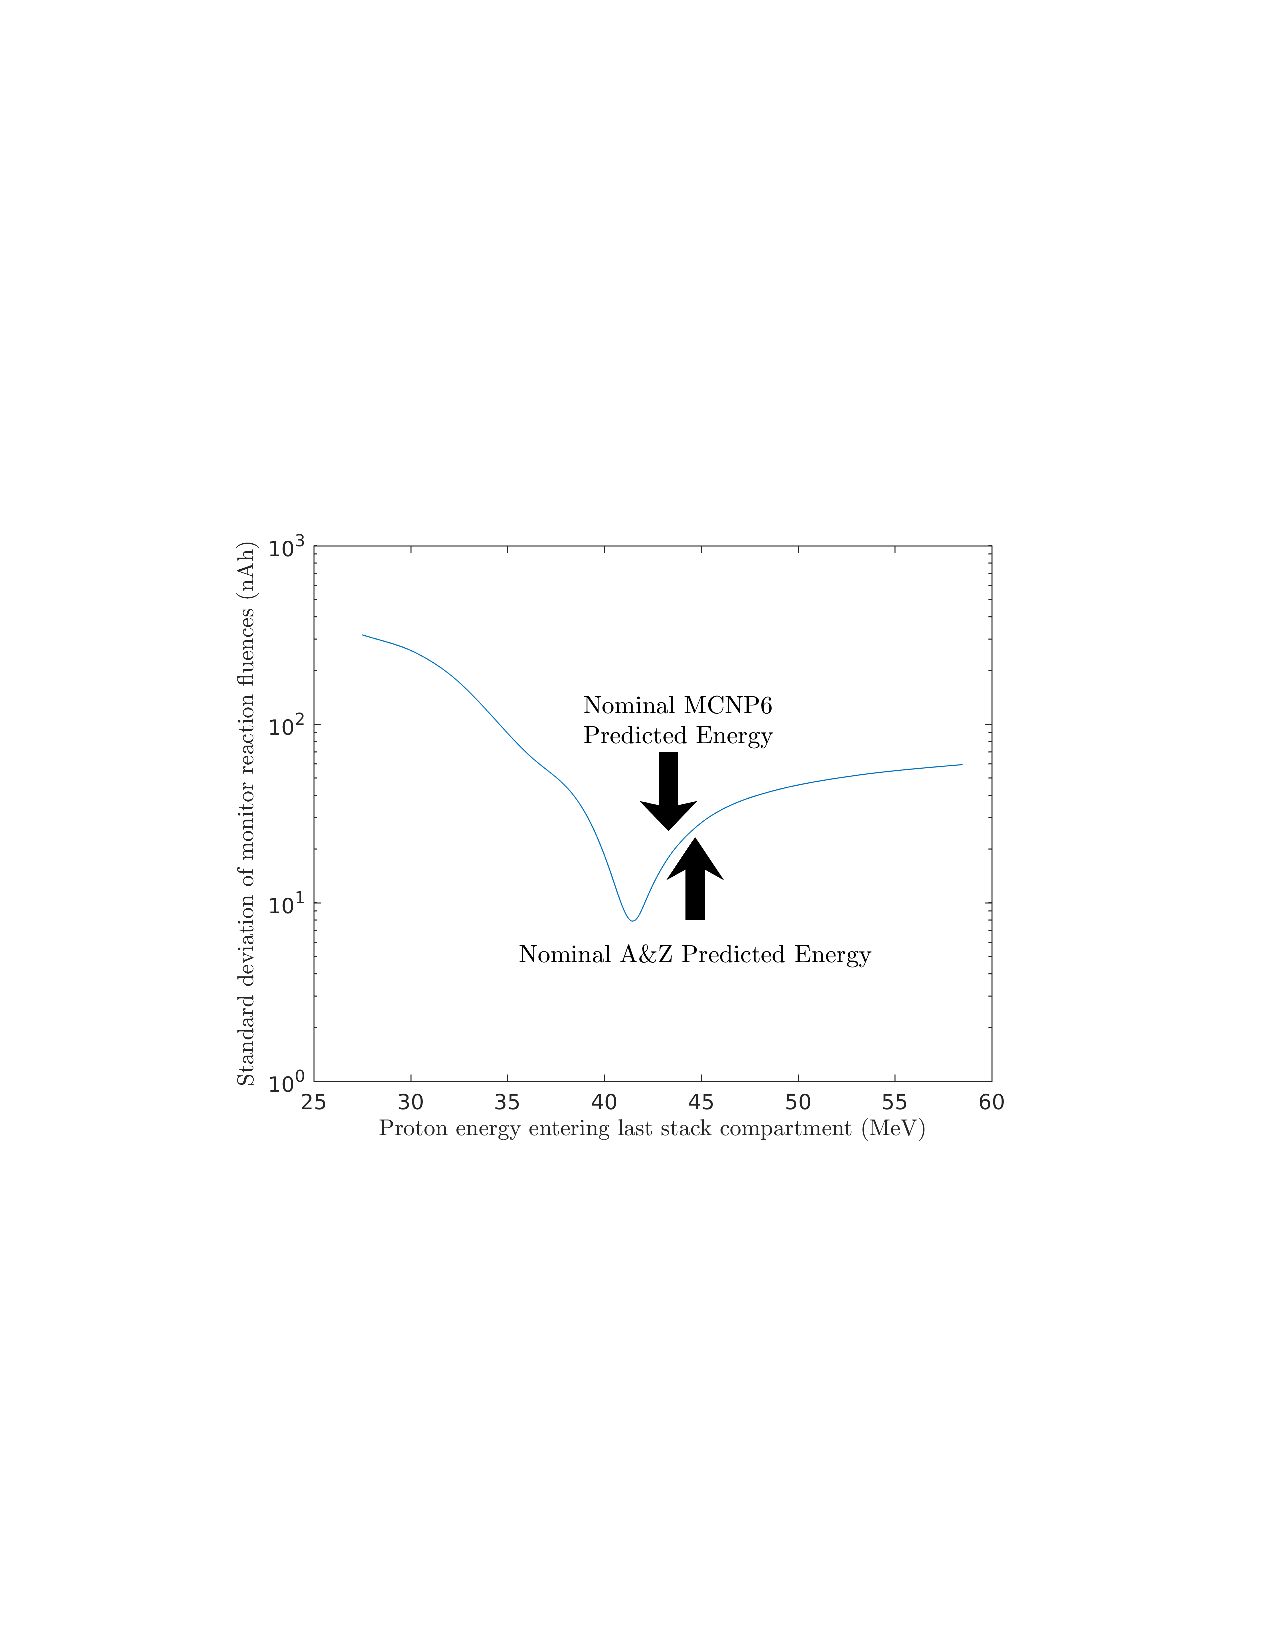
\includegraphics[clip=true,trim=1.5in 3.4in 1.8in 3.5in, scale=0.8]{./figures/variation_curve.pdf}
 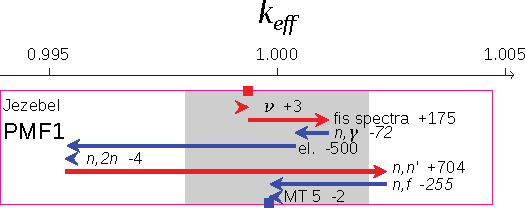
\includegraphics[width=0.8\linewidth]{rotated_swings.pdf}

 % variation_curve.pdf: 612x792 pixel, 72dpi, 21.59x27.94 cm, bb=0 0 612 792
 \caption{Simulations of criticality $k_{eff}$ for \ce{^{239}Pu} for the fast assembly Jezebel, PMF-1. This figure shows that both LANL CIELO-1 (ENDF/B-VIII.0) and CEA CIELO-2 (JEFF-3.3) predict similar $k_{eff}$ values, but do so for very different reasons. The changes in criticality are evident when individual cross section channels are substituted between the two evaluations.  The shaded region shows the  resulting range of values for $k_{eff}$.}
 \label{fig:rotated_swings}
\end{figure}

A new Collaborative International Evaluated Library Organization (CIELO) Coordinated Research Program was started under the auspices of the IAEA \cite{Cha18a} to have the international nuclear data evaluation community agree on a set of evaluated cross sections and output spectra for six critically-important nuclei: \ce{^{1}H}, \ce{^{16}O}, \ce{^{56}Fe}, \ce{^{235,238}U} and \ce{^{239}Pu} in order to address the issue of compensating errors.  Recently, this list has been expanded to include \ce{^{14,15}N}, \ce{^{9}Be}, \ce{^{23}Na}, \ce{^{59}Co}, \ce{^{58}Ni}, \ce{^{238-242}Pu}.

CIELO has relatively little energy or angle differential data to draw upon to aid in its evaluation of (n,n') on the \enquote{Big 3} Actinides, leading to \enquote{significant differences amongst the evaluations for \ce{^{239}Pu} in the fast energy range, with ENDF/B-VII.1 and JENDL-4.0 lying significantly above the JEFF-3.1 evaluation.} \cite{Cha14}.  The \ce{^{239}Pu} data referenced in their paper are all from indirect measurements made prior to 1970 \cite{Batchelor1969, Andreev1961}.  The case is similar for \ce{^{235}U} where they note that differences for $E_n >$ 50 keV \enquote{have a large impact on the fast criticality (Godiva), leading to a 540 pcm swing in calculated criticality, as shown by Go Chiba \cite{Chi12}.}

One significant source of (n,xn$\gamma$) partial cross section data from 1997 to 2003 was the GEANIE collaboration (Germanium Array for Neutron-Induced Excitations) at the Los Alamos Neutron Science Center/Weapons Neutron Research (LANSCE/WNR) facility. While the primary goal of the GEANIE collaboration was the determination of the \ce{^{239}Pu}(n,2n) cross section \cite{Ber02}, it resulted in the publication of more than two dozen papers over the course of more than 15 years.  Experiments were run on all three of the major Actinides: \ce{^{235}U} \cite{You01}, \ce{^{239}Pu} \cite{Ber02} and \ce{^{238}U} \cite{Fot04}.  It should be noted that GEANIE did not include any neutron detectors, producing only angle-integrated partial $\gamma$-ray cross sections.  

The need for new scattering data has motivated many new experiments.  This has included energy-differential/angle-integrated measurements of the \ce{^{238}U}(n,n') cross section using the GELINA spallation neutron source in Geel Belgium by Bacquias et al., \cite{Nem13} and quasi-angle-differential measurements using the Rensselaer Polytechnic Institute Linac by Daskalakis et al., \cite{Das14}. 

The ideal way to improve (n,n') data on the \ce{^{235,238}U} and \ce{^{239}Pu} would be to perform measurements of the scattered neutron in coincidence with transitions emitted by the excited nucleus.  In the case of the Actinides this will potentially require the observation of conversion electrons given that the lowest transitions in all actinides are almost entirely converted.  Unfortunately, neutron beams usually have quite low intensity, with a fluence in the fast (1--10 MeV) region between $10^3$ and $10^7$ n/s/cm$^2$ at the target location.  Furthermore, many spallation neutron sources have a significant high-energy spectral component that can cause inter-element scattering in a neutron scintillator array rendering precise determination of the scattered neutron energy difficult to  perform. However, intense limited-energy neutron sources based on thick-target deuteron breakup \cite{Harrig2018} and forward-fitting techniques developed for use at spallation neutron sources \cite{Kee18} offer an opportunity to perform neutron-gamma coincident measurements in the fast fission energy spectrum.  These techniques could provide valuable data to improve nuclear data evaluations of inelastic scattering, even on targets where fission is an open channel. 

\subsection{Improved treatment of continuum nuclear data properties}

Information regarding states in the unresolved continuum region above the particle separation energy is of central importance to accurately modeling the competition between particle and gamma-ray emission.  The most important of these are the nuclear level density (NLD) as a function of energy, spin and parity, and the radiative strength function (RSF), which describes the ability of excited nuclear matter to absorb or emit photons.  A number of recent studies have shown the importance of the RSF to modeling (n,$\gamma$) reactions for neutrons with energies between 1 and 100 keV, which corresponds to the spectrum at the site of neutron capture nucleosynthesis in stars \cite{PhysRevC.82.014318, Lar15} and energy generation in fast reactors and nuclear security applications.   

Over the past several years, work led by the group at the University of Oslo has shown that there is a surprisingly large amount of M1 radiative strength believed to be a type of \enquote{scissors} collective mode throughout the Actinide mass region near the valley of stability including \ce{^{238}U}, \ce{^{239,240,242}Pu} and \ce{^{232}Th} \cite{Lap16, Gut13, Gut13a, Gut14, Gut15}.

Other results from the Oslo group show that Actinide NLDs appears to follow a constant temperature (CT) form with a roughly Gaussian dependence on angular momentum that is often described via an energy-dependent width spin cut-off parameter ($\sigma$) of the form: 
\begin{equation}\label{eqn:spin_cutoff}
\sigma\pp{E_x}=0.01389 \dfrac{A^{5/3}}{\widetilde{a}}\sqrt{aU}
\end{equation}
where $U$ is roughly the $E_x$ minus the pairing gap $\Delta$, $a$ is the level density parameter, $A$ is the nuclear mass and $\widetilde{a}$ is the asymptotic level density value one would obtain in the absence of any shell effects. 

There is a great deal of uncertainty in the magnitude of the spin cut-off parameter.  This is a significant issue since a good knowledge of the $J$ distribution is needed to accurately model the neutron vs. $\gamma$-ray emission probability in nuclear reactions.  This sensitivity was shown recently by Wiedeking et al., \cite{Wie16} who showed that neutron emission from excited states in \ce{^{95}Mo} well-above the neutron separation energy populated via (d,p) was hindered for states with high angular momentum. 



\begin{figure}
 \centering
%  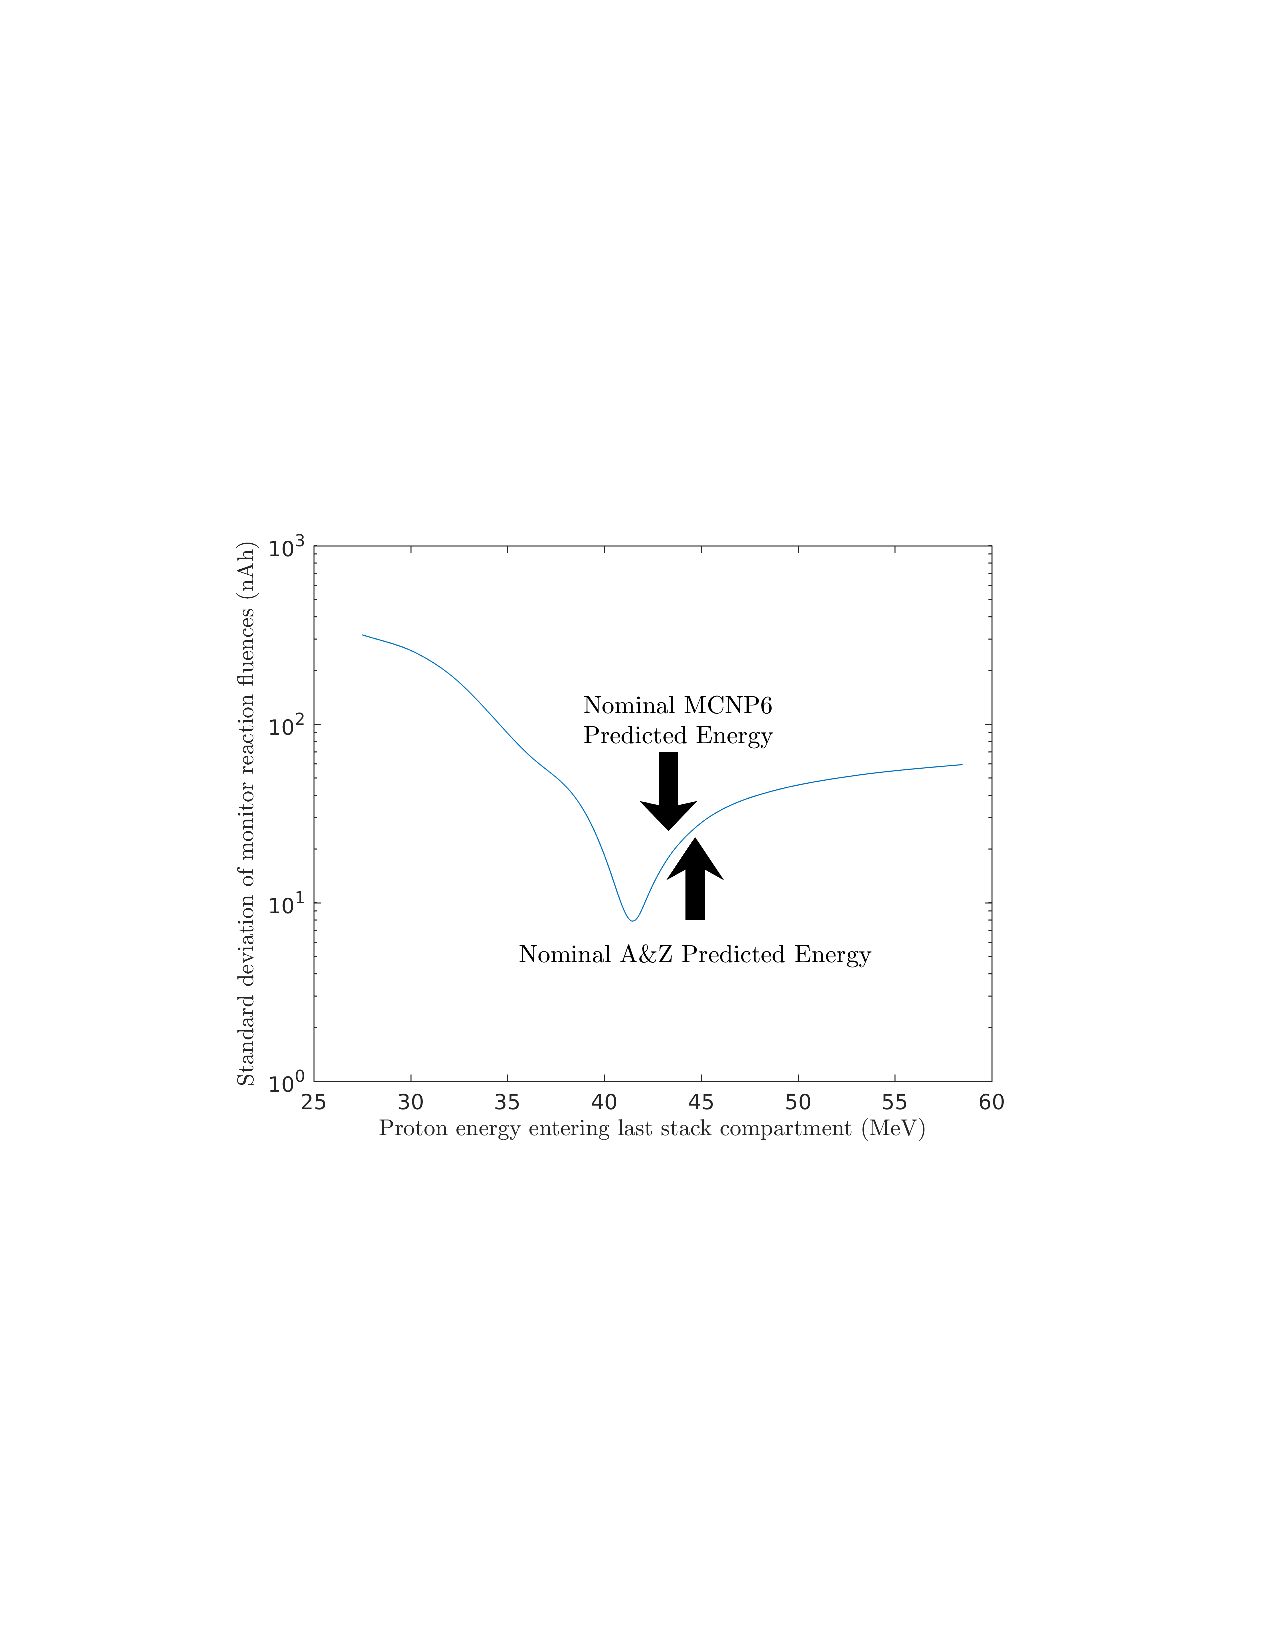
\includegraphics[clip=true,trim=1.5in 3.4in 1.8in 3.5in, scale=0.8]{./figures/variation_curve.pdf}
 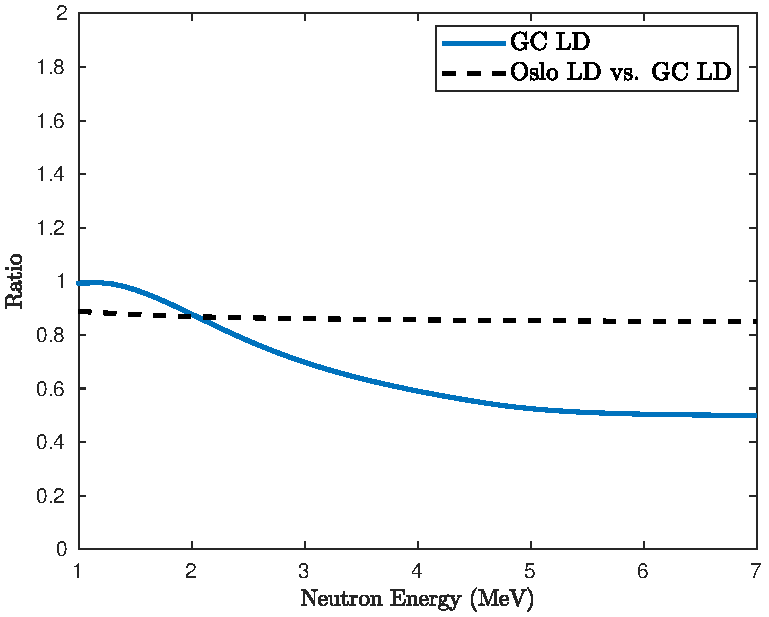
\includegraphics[width=0.7\linewidth]{fig3.pdf}

 % variation_curve.pdf: 612x792 pixel, 72dpi, 21.59x27.94 cm, bb=0 0 612 792
 \caption{Ratio of the \ce{^{238}U}(n,n') cross section to the state calculated using TALYS for two different sets of input parameters as a function of incident neutron energy. The solid line shows the ratio where spin cutoff has been scaled to $\pm$25\% of its default value. The dashed line shows the case where the default value calculated using LD Model 1 (Gilbert and Cameron) is divided by the value obtained using the data from Guttormsen \cite{Gut13a}.}
 \label{fig:oslo_ld_plot}
\end{figure}



(n,n'$\gamma$) provides a useful tool for studying the spin cut-off parameter since the reactions proceed largely through the population of a compound nucleus with a relatively wide range of angular momentum. \autoref{fig:oslo_ld_plot} shows the ratio of the partial cross section for the population of the  level in \ce{^{238}U}(n,n') as a function of incident neutron energy calculated using the TALYS reaction code for two different choices of spin cut-off.  The solid line shows the case where a constant temperature level density is assumed and the spin cut-off parameter was varied from 75\% to 125\% of its \enquote{normal} value given by \autoref{eqn:spin_cutoff} above.  The ratio decreases by nearly a factor of 2 with increasing energy.  In contrast, the dashed line shows the ratio of the  population of the  state when the LD and RSF from the recent Oslo measurements \cite{Gut13a} is divided by the results obtained using the default Gilbert and Cameron in TALYS.  In this case the ratio decreases by nearly a factor of 2.  Similar behavior is seen in the partial cross sections for other off-yrast levels as well. 


\begin{figure}
    \centering
    \begin{minipage}{0.5\textwidth}
        \centering
        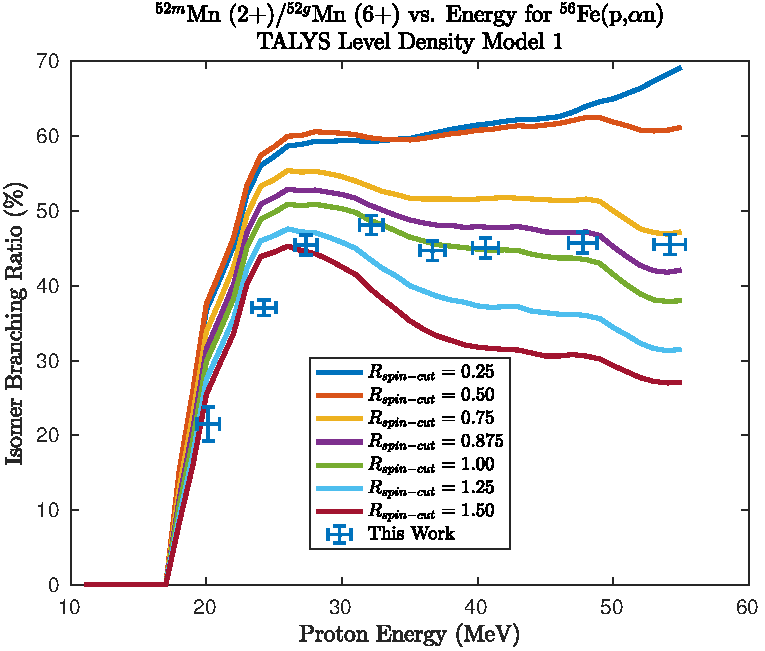
\includegraphics[width=0.97\textwidth]{isomer_curves.pdf} % first figure itself
%         \caption{first figure}
    \end{minipage}\hfill
    \begin{minipage}{0.5\textwidth}
        \centering
        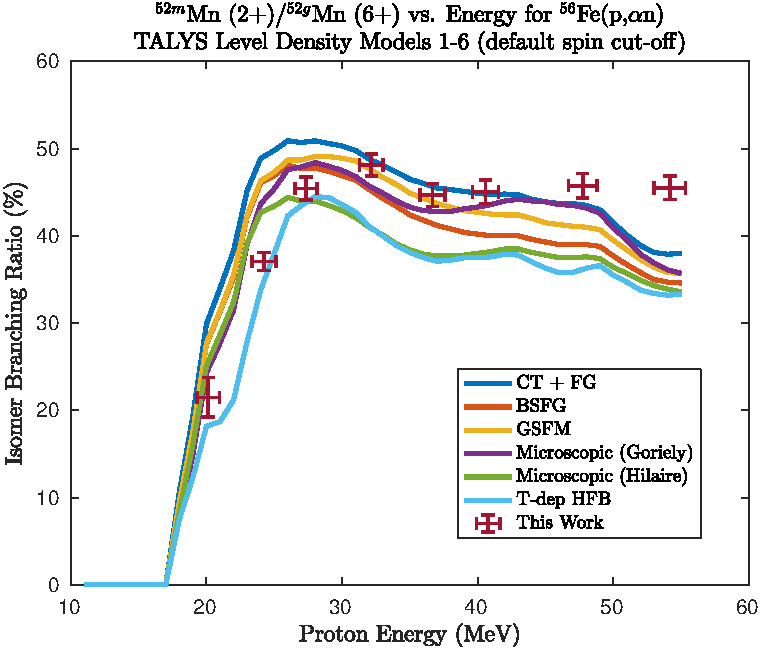
\includegraphics[width=0.97\textwidth]{ldmodels.pdf} % second figure itself
%         \caption{second figure}
    \end{minipage}
    \caption{Predictions of the production of \ce{^{52m}Mn}($J_\pi=2^+$)/\ce{^{52g}Mn}($J_\pi=6^+$) isomer-to-ground state ratio as a function of energy for the Gilbert and Cameron level density (left) and using the 6 level density models available in TALYS (right). }
     \label{fig:fe_isomer_plots}
\end{figure}


% \begin{figure}
%     \centering
% %     \subfloat{
% %         \centering
% %         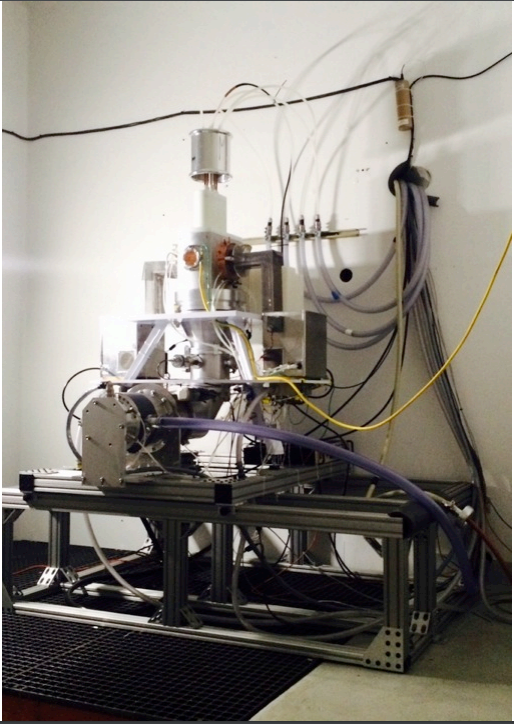
\includegraphics[width=\columnwidth]{./figures/Capture.PNG}
% %         \hspace{-5pt}
%         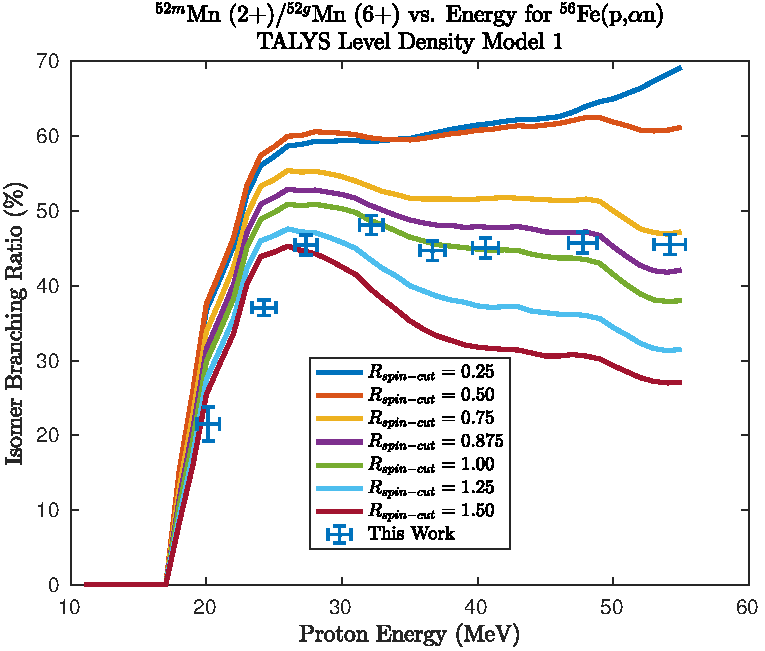
\includegraphics[width=0.3\textwidth]{isomer_curves.pdf} 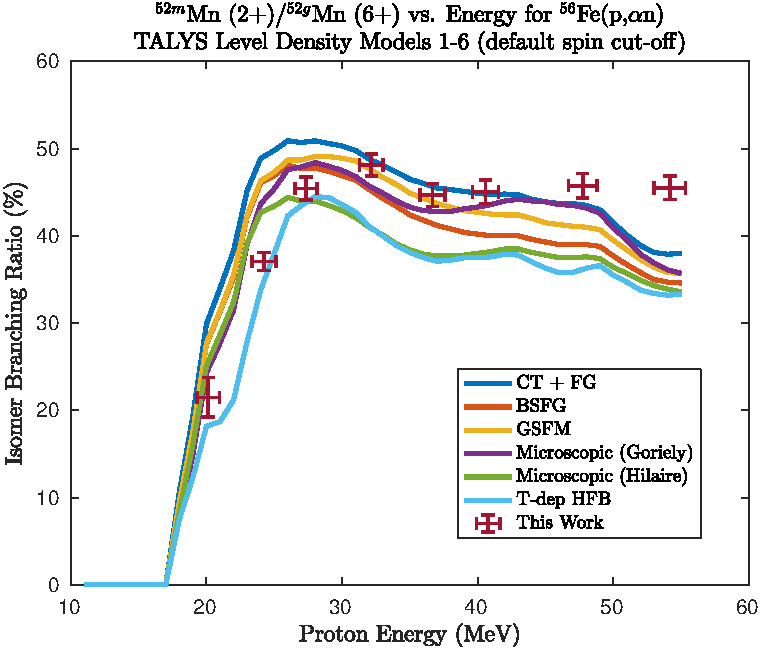
\includegraphics[width=0.3\textwidth]{ldmodels.pdf}
% %         \caption{ Decay curve for the isomeric transition of \ce{^{115m}In}.}
%          %         \refstepcounter{subfigure}
% %          \label{fig:before_minimization}
% %    \hspace{-5pt}%
% %      \subfloat{
% %         \centering
% %         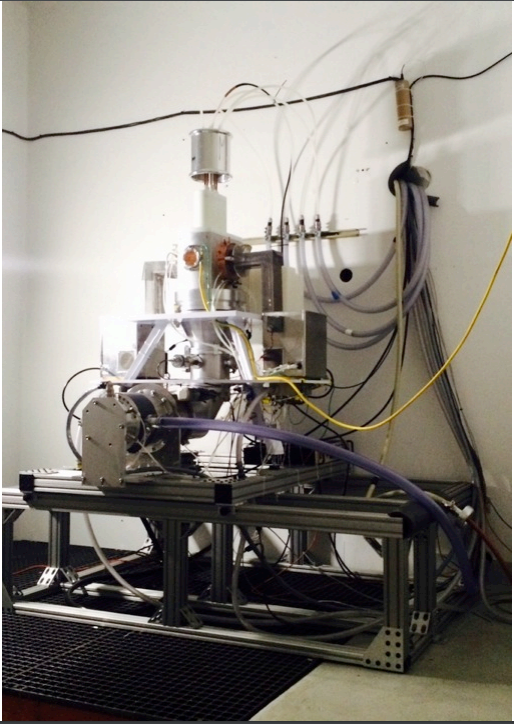
\includegraphics[width=\columnwidth]{./figures/Capture.PNG}
% %         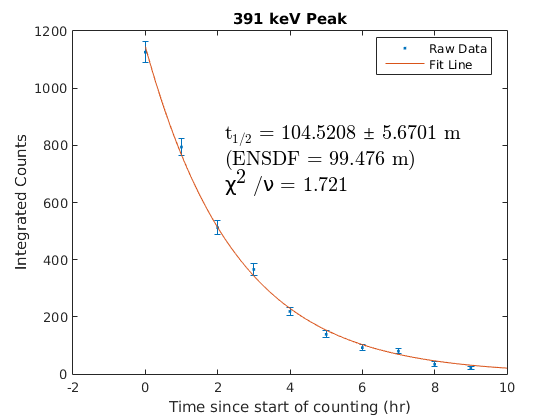
\includegraphics[scale=0.6]{./figures/391keV_curve2.png}
% %         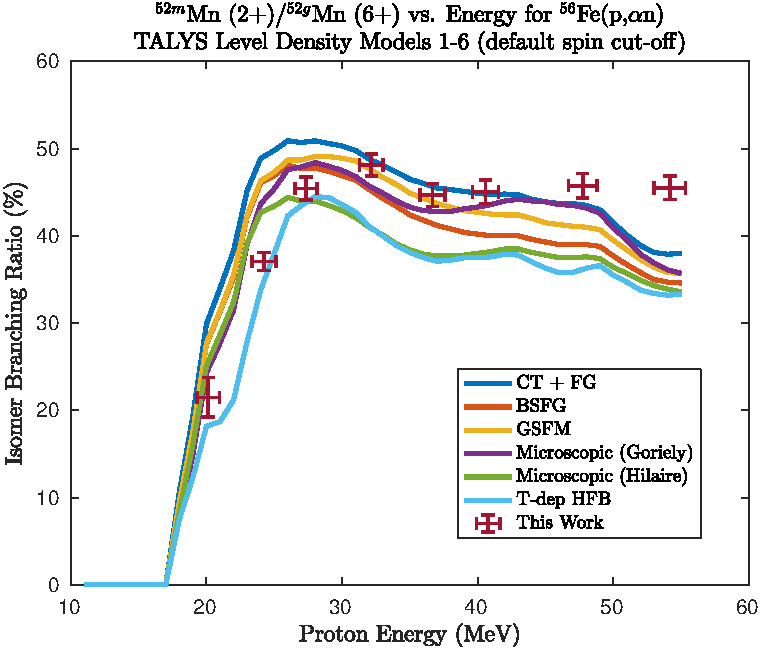
\includegraphics[width=0.3\textwidth]{ldmodels.pdf}
% %         \caption{ Decay curve for the isomeric transition of \ce{^{113m}In}.}
%          %         \refstepcounter{subfigure}
% %          \label{fig:after_minimization}
% %    \hspace{-5pt}%
%     \caption{Predictions of the production of \ce{^{52m}Mn}($J_\pi=2^+$)/\ce{^{52g}Mn}($J_\pi=6^+$) isomer-to-ground state ratio as a function of energy for the Gilbert and Cameron level density (left) and using the 6 level density models available in TALYS (right). }
%      \label{fig:fe_isomer_plots}
% \end{figure}

Information regarding the $J$-dependence of the NLD can also be obtained through observation of the relative population of two low-lying states with very different spins via activation.  This method has been used in Hg and Au by Chakravarty \cite{PhysRevC.45.1171} and more recently by Sudar in Hg and Pt \cite{PhysRevC.73.034613}.  \autoref{fig:fe_isomer_plots} shows this for the case of \ce{^{52m}Mn}($J_\pi=2^+$)/\ce{^{52g}Mn}($J_\pi=6^+$) ratio populated via \ce{^{56}Fe}(p,$\alpha$n) measured via stacked-target activation at the LBNL 88-Inch cyclotron as compared to TALYS calculations for different values of the spin cut-off parameter (left) and the 6 level density models available for use in TALYS on the right.  


It should be noted that both the (n,n'$\gamma$) and isomer-to-ground state ratio measurements could be performed as part of a program that supports improved neutron transport as described in \autoref{sec:n_transport} above, and a program of cross section measurements in support of medical isotope production described in \autoref{sec:isotope_production} below.  This reflects the interdependency between nuclear data over a wide range of applications.  


\section{NATIONAL SECURITY AND NON-PROLIFERATION}



\subsection{Interpreting the reactor anti-neutrino spectrum}

One canonical example of a non-proliferation activity where improvements in multiple cross-cutting areas of nuclear data are needed is the interpretation of the anti-neutrino spectrum from the prompt decay of fission fragments in the core of a nuclear reactor. Nuclear reactors are prolific sources of electron antineutrinos, producing about $10^{21}$ antineutrinos per second for a typical power reactor.  These electron antineutrinos are produced by the beta-minus decay of the more than 800 neutron-rich fission fragments, which are the debris from the main source of energy generation in a reactor, the neutron induced fission of actinide nuclides.  These antineutrinos are also the only radiation escaping from the vessel of a safely operating nuclear reactor, making them ideally suited for reactor monitoring, even in the event that the actor operating the reactor refuses to cooperate with the international community.  Recent technological advancements in electron antineutrino detection has made another dream a reality, monitoring the performance of nuclear reactors and tracking \ce{^{239}Pu} for non-proliferation treaty verification.   The WATCHMAN experiment in the UK has just started to explore this field \cite{Cha18}.  Furthermore, the possible use of antineutrino detectors for the detection of nuclear explosions has been discussed \cite{CarAx}.
 
Nuclear reactors have also been an essential tool to study the weak interaction.  Their large antineutrino flux was capitalized by Cowan and Reines to discover antineutrinos in 1956 \cite{Cow56}, more than 25 years after they were first hypothesized by Pauli in 1930 to explain the continuum electron spectra observed following beta-minus decay.   In the last few years, the transformation of electron antineutrinos into the other two flavors was beautifully measured by three large-scale experimental efforts, Daya Bay \cite{An16}, Double Chooz \cite{Abe12} and RENO \cite{Cho16}.   These experiments also confirmed a deficit of antineutrinos of about 5--9\% at short distances that had been revealed in a 2011 re-analysis of the conversion procedure to obtain antineutrino spectra from the measured electron spectra \cite{Men11}.

This intriguing deficit, as well as a spectrum distortion, has triggered a new generation of very-short distance reactor experiments, such as NEOS (Korea) \cite{Ko17}, DANSS (Russia) \cite{AleAx}, STEREO (France) \cite{AllAx}, PROSPECT (USA) \cite{Ash16}, and SoLid (Belgium) \cite{Kal17}, whose first results are beginning to be made public.  There are no signs of slowing down in the field of nuclear reactor antineutrinos, as the largest experiment to date, JUNO, designed to measure the neutrino mass hierarchy, should be ready for data taking by 2021 \cite{SalAx}.  JUNO will feature a 20 Million-Ton detector at 80 km from A 27 GW nuclear power plant in China.

The antineutrino spectrum produced in a nuclear reactor is calculated as the sum of the spectra produced by each of the nuclear fuels, \ce{^{235,238}U} and \ce{^{239,241}Pu}, weighted by the respective fission fractions \cite{Vog81}.   The spectra for each fuel can be calculated using nuclear databases, in what is commonly known as the \enquote{summation method}.   Alternatively, for \ce{^{235}U} and \ce{^{239,241}Pu}, the spectra can also be calculated by converting the aggregate electron spectra measured at ILL in the 1980s \cite{Fei82,Sch85,Hah89}.   The current best predictions for  \ce{^{235}U} and \ce{^{239,241}Pu} are those by Huber \cite{Hub11} using the conversion method, while for \ce{^{238}U} is that by Mueller et al. \cite{Mue11} using a hybrid conversion-summation method.

The use of nuclear databases to calculate antineutrino spectra is considered less precise than the conversion method due to deficiencies in the underlying fission and decay data, such as beta intensities \cite{Fal12}, beta shape factors due to first-forbidden transitions \cite{Hay14}, evaluated libraries issues \cite{Son15} and fission yields \cite{Son16}.   There have been considerable efforts in the last few years to improve this situation, including (i) experimental campaigns in Jyvaskyla \cite{Alg10}, ORNL \cite{Ras16} and ANL \cite{MccTBD} to obtain highly precise values of beta intensities, which have been incorporated in the ENDF/B-VIII.0 decay data sub-library; (ii) measurements of isomeric ratios in ILL, Jyvaskyla and ANL; (iii) measurements of fission yields in GELINA \cite{Viv00}, GSI \cite{Pel17} and LANL \cite{Duk16}; (iv) a recent IAEA Coordinated Research Project on beta-delayed neutron emitters \cite{DimXX} that would improve the derivation of cumulative fission yields from independent ones.   Also planned are measurements of beta shape factors as well as a new IAEA Coordinated Research Project to evaluate fission yields.
Another issue affecting the summation method is the lack of fission yield correlation matrices in the evaluated fission data libraries.   As a result, uncertainties cannot be fully computed.  There has been some progress in this area, for instance, the ongoing OECD-NEA subgroup 44 will incorporate this topic \cite{SobXX}.

The summation method has been recently applied in two different situations.   First, it has been shown that the Daya Bay fuel evolution data \cite{An17} can be explained by summation calculations including an anomaly of about 4\% \cite{Hay18}.   Second, a novel method to analyze the Daya Bay spectrum revealed the signature of 4 individual fission products, while the same method applied to the electron spectra revealed two additional fission products \cite{Son18}.   

The conversion method is not fully free of issues, either.  To start, it is based on a single set of measurements; also, its most basic premise, the description of a level-to-level spectrum using a particular formalism, has not been tested, as highly precise measurements of electron spectra for fission products above the inverse beta decay cross section threshold have not been published.    As a result, while more precise than the summation method, it is nevertheless considerably less reliable.     A recent article \cite{Son17} reviewed the different Fermi functions available for the calculation of spectra and showed that a linear correction factor of 6\%/MeV could explain the anomaly.

Given the dependence of the antineutrino signal on both decay and fission product yield data, a series of sensitivity study-guided integral experiments, along the lines of critical assembly integral benchmarks, are needed to validate the underlying nuclear data would provide a strong constraint on the underlying data.  One approach would involve irradiating fissile and fissionable samples in facilities with well-understood neutron spectra and comparing the observed delayed gamma-rays to a modeled spectrum produced using the Fission Induced Electromagnetic Response (FIER) code developed at Berkeley \cite{Matthews2018}.  FIER convolves fission product yield distributions and decay data to predict the gamma-ray spectrum after neutron irradiation.  The first example of its use involving a comparison to the delayed gamma-ray spectrum from a \ce{^{235}U} foil irradiated in the Godiva critical assembly indicated several cases were the underlying fission yields or decay data required improvement. 

\textred{We seem to have plenty of space - should we add the FIER plot back in?}

These experiments would involve a sample of depleted \ce{^{238}U} since recent results from IBD indicate that the contribution to the observed anomaly in the antineutrino experiment can be attributed to issues with the \ce{^{238}U}(n,f) yields. These measurements could be performed at the Godiva in the same fashion as the \ce{^{235}U} irradiation used to validate FIER, or other well-documented fast neutron facilities including the thick target deuteron break neutron source at the LBNL 88-Inch cyclotron \cite{Harrig2018} and the High Flux Neutron Generator at UC-Berkeley \cite{ayllon2018design} and compare the results to the FIER predictions to inform both the fission yield and decay data for \ce{^{238}U}(n,f). 

\subsection{Improved (n,x\texorpdfstring{$\gamma$}{ gamma}) data for active interrogation}

An invaluable tool for determining the presence of fissile materials for non-proliferation involves prompt neutron- and gamma-ray spectroscopy coupled to a DT neutron source with associated particle imaging (DT-API).   DT-API sources allow tracking of the trajectory of individual neutrons, thereby greatly decreasing background from scattered neutrons.  The signal from DT-API generators includes long-chain gamma-ray emission from multiple fission events \cite{Pra12,Nak10} as well as prompt gamma- and neutron scattering on a wide range of low- and high-Z materials.   

The interpretation of this data requires detailed knowledge of both the double-differential neutron scattering and gamma-ray production cross sections from fast down to thermal neutron energies.  The Evaluated Gamma Activation File \cite{Fir15} provides partial gamma-ray cross section data for transitions between discrete states following thermal neutron capture.  At higher energies the Atlas of Gamma-rays from the Scattering of Reactor Fast Neutrons \cite{Dem78}, which has recently been compiled into a database and reconciled to reflect state-of-the-art gamma-ray energies from ENSDF \cite{Hur18}, offers discrete gamma-ray cross sections for irradiation with fast fission neutrons.  

A program of measurements of gammas emitted from both discrete and QC states would require a relatively modest effort to set in place.  The data from these measurements could then be used to guide physics-based reaction model, such as the COH, TALYS or EMPIRE to ensure that the total gamma-ray production cross section is consistent with the total capture and scattering cross sections themselves. 


\section{ISOTOPE PRODUCTION}\label{sec:isotope_production}


The high energy density and wide range of decay lifetimes and chemical properties of radionuclides near the nuclear valley of stability make them an extremely versatile tool for applications ranging from the diagnosis and treatment of illness, to nuclear non-proliferation and environmental studies, to powering spacecraft to explore the outer reaches of the solar system and beyond. Furthermore, given that there are hundreds of unstable nuclei with lifetimes in excess of 1 hour and less than 100 years between Hydrogen and Californium, it is clear that we have barely scratched the surface of potential applications.

However, there are significant uncertainties in both the reactions used to produce these radionuclides and/or the intensities and energies of their decay radiation.  There have been numerous papers produced over the past 5 years detailing some of the nuclear data needs associated with producing radionuclides for applications. For a comprehensive listing of nuclear data needs associated with radionuclides we refer the reader to the summary whitepaper from the Nuclear Data Needs and Capabilities for Applications Workshop held in Berkeley in 2015 \cite{bernstein2015nuclear}, particularly the reactions and isotopes listed in Appendix B.  Additional guidance regarding nuclear data needs for medical isotopes can be found in a recent series of IAEA studies \cite{Iae675,Iae596,Iae591} as well as an exhaustive paper from Qaim et al. \cite{Qaim201731}.

Over 20 million nuclear medicine procedures are performed each year in the United States \cite{Met09}, with the vast majority involving imaging.  \ce{^{99m}Tc} ($t_{1/2}$ = 6.0067(5) hour), which decays predominately via the emission of single 140 keV gamma-ray, is used in 80\% of of these procedures. \ce{^{99m}Tc} is produced via \ce{^{235}U}(n,f).  However, this approach is less than ideal due to the increasing age of many reactors \cite{Qai12} and a nuclear weapons proliferation risk associated with reactors utilizing Highly-Enriched Uranium (HEU).  As a result, alternative \ce{^{99m}Tc} production pathways, as well as studies of the associated production of long-lived impurities \cite{Updegraff2013}, are under consideration \cite{Rut09}. 


Other imaging radionuclides are used in Positron Emission Tomography (PET), which is now so commonplace that
there are numerous companies   providing production capabilities built around low-energy \enquote{medical cyclotrons.} 
The utility of PET imaging, combined with the recent rise in multimodal PET/MRI and PET/CT imaging,  has
led to significant interest in the development of other $\beta^+$ emitting radionuclides.
These include \ce{^{18}F} ($t_{1/2}$ = 109.771(20) min), which is produced locally via the \ce{^{18}O}(p,n) reaction, \ce{^{82}Rb} ($t_{1/2}$ = 1.2575(2) min), which is used in cardiac imaging, and \ce{^{68}Ga}  ($t_{1/2}$ = 67.71(8) min), which is used in the detection of a wide range of tumors.  The short half-lives of \ce{^{82}Rb} and \ce{^{68}Ga} necessitate that they be extracted from a longer-lived radioactive parent nuclide generator whose longer half-lives of 270.93(13) and 25.35(3) days, respectively, allow them to be produced at regional facilities and distributed to medical facilities throughout the world.  

In addition to imaging, a large number of therapeutic radiopharmaceuticals are in use or under development for cancer treatment.  The principle behind therapeutic radionuclide cancer therapy involves depositing a targeted dose, e.g., energy per unit mass, to a tumor cell,  capable of producing damage to multiple strands of DNA, from which the cell cannot recover.  The ideal dose delivery involves radiation with a high Linear Energy Transfer (LET).  While some $\beta^-$ nuclides are already in use, such as \ce{^{177}Lu} ($t_{1/2}$ = 6.6475(20) days), the relatively long range of $\beta^-$-particles makes them less favorable than other modes of radioactive decay.  These include Auger/Coster-Kronig electron-emitters, which typically have a range of less than 1 \mmicro m, or $\alpha$-particle emitters, which have ranges of 2--10 \mmicro m.  

There is a particularly large amount of interest in the alpha-emitting radionuclide \ce{^{225}Ac}.  \ce{^{225}Ac} is particularly well-suited for medical applications in that it has a sufficiently long lifetime ($t_{1/2}$ = 10.0(1) days) to facilitate its incorporation into targeting molecules, and its daughters then decay relatively rapidly ($t_{1/2}<$ 3.2 hours) to stable products, minimizing concurrent dose to healthy tissue. Other promising alpha-therapeutic radionuclides include \ce{^{211}At}, \ce{^{212}Pb}/\ce{^{212}Bi}, \ce{^{213}Bi}, \ce{^{226}Th} and \ce{^{227}Th}, and have all been identified as high priority topics by the most recent Nuclear Science Advisory Committee's Long Range Plan on Isotope Production \cite{NSACIsotopesSubcommittee2015}.

A particularly promising  nuclear medical treatment modality involves coupling a pair of chemically similar radioisotopes including of a therapeutic nuclide capable of delivering a highly localized radiation dose and a chemically-identical isotope that emits a positron for PET or a gamma suitable for single photon emission computed tomography (SPECT) imaging.
Examples of these \enquote{theranostic pairs} include \ce{^{188}Pt} or \ce{^{191}Pt} for use in imaging, together with \ce{^{193m}Pt}, \ce{^{195m}Pt}, and \ce{^{197}Pt}, which all have  therapeutic potential.
Another such promising  pair involves the PET isotope \ce{^{134}Ce} ($t_{1/2}$ = 3.16(4) days) combined with \ce{^{225}Ac}.  A recent NSAC report \cite{NSACIsotopesSubcommittee2015} highlights additional pairs of isotopes that have potential uses as theranostic agents. 

As mentioned above, most of these promising radionuclides are made at a few regional facilities.  These include the Isotope Production Facility at Los Alamos National Lab (IPF-LANL), the Brookhaven Linac Isotope Production facility at Brookhaven National Lab (BLIP-BNL) in the United States, the TRIUMF laboratory in Canada and iThemba LABS in South Africa \cite{Iae675,NSACIsotopesSubcommittee2015}.  In a compelling example of the synergy between fundamental nuclear research and societal benefit, LANL-IPF and BLIP-BNL operate symbiotically with the Los Alamos Neutron Science Center at LANL and the Relativistic Heavy Ion Collider at BNL.  This dual-use approach provides an inexpensive, reliable source of radionuclides needed for the development of new drugs through a public-private partnership. 

All of these regional sources utilize high-energy ($\geq$ 100 MeV) (p,x) reactions on stable targets.  In addition to producing the radionuclides of interest these reactions create a large flux of \enquote{secondary} spallation protons and neutrons that can in turn initiate nuclear reactions providing either a useful alternative source of valuable radionuclide or a troublesome chemically-identical contaminant.  The secondary neutron flux is particularly important since the lack of electronic stopping for neutrons makes them advantageous for radionuclide production \cite{Voyles2017}.  The energy spectrum of secondary neutrons from IPF was recently measured using spectral unfolding \cite{Mos16} and for thick-target deuteron break-up on beryllium at the LBNL 88-Inch cyclotron \cite{Harrig2018} via a secondary time-of-flight technique. A number of therapeutic radionuclides can potentially be produced via secondary neutron-induced (n,p) reactions. Examples of possible targets include \ce{^{32}S}, \ce{^{47}Ti}, \ce{^{nat}Zn} (for the production of \ce{^{64,67}Cu}), \ce{^{105}Pd}, \ce{^{149}Sm}, \ce{^{175}Lu}, and \ce{^{177}Hf}.  In addition, the production of alpha-emitting radionuclides such as \ce{^{225}Ac}, \ce{^{223}Ra}, and \ce{^{227}Th} using neutrons has yet to be explored.


\begin{figure}
 \centering
%  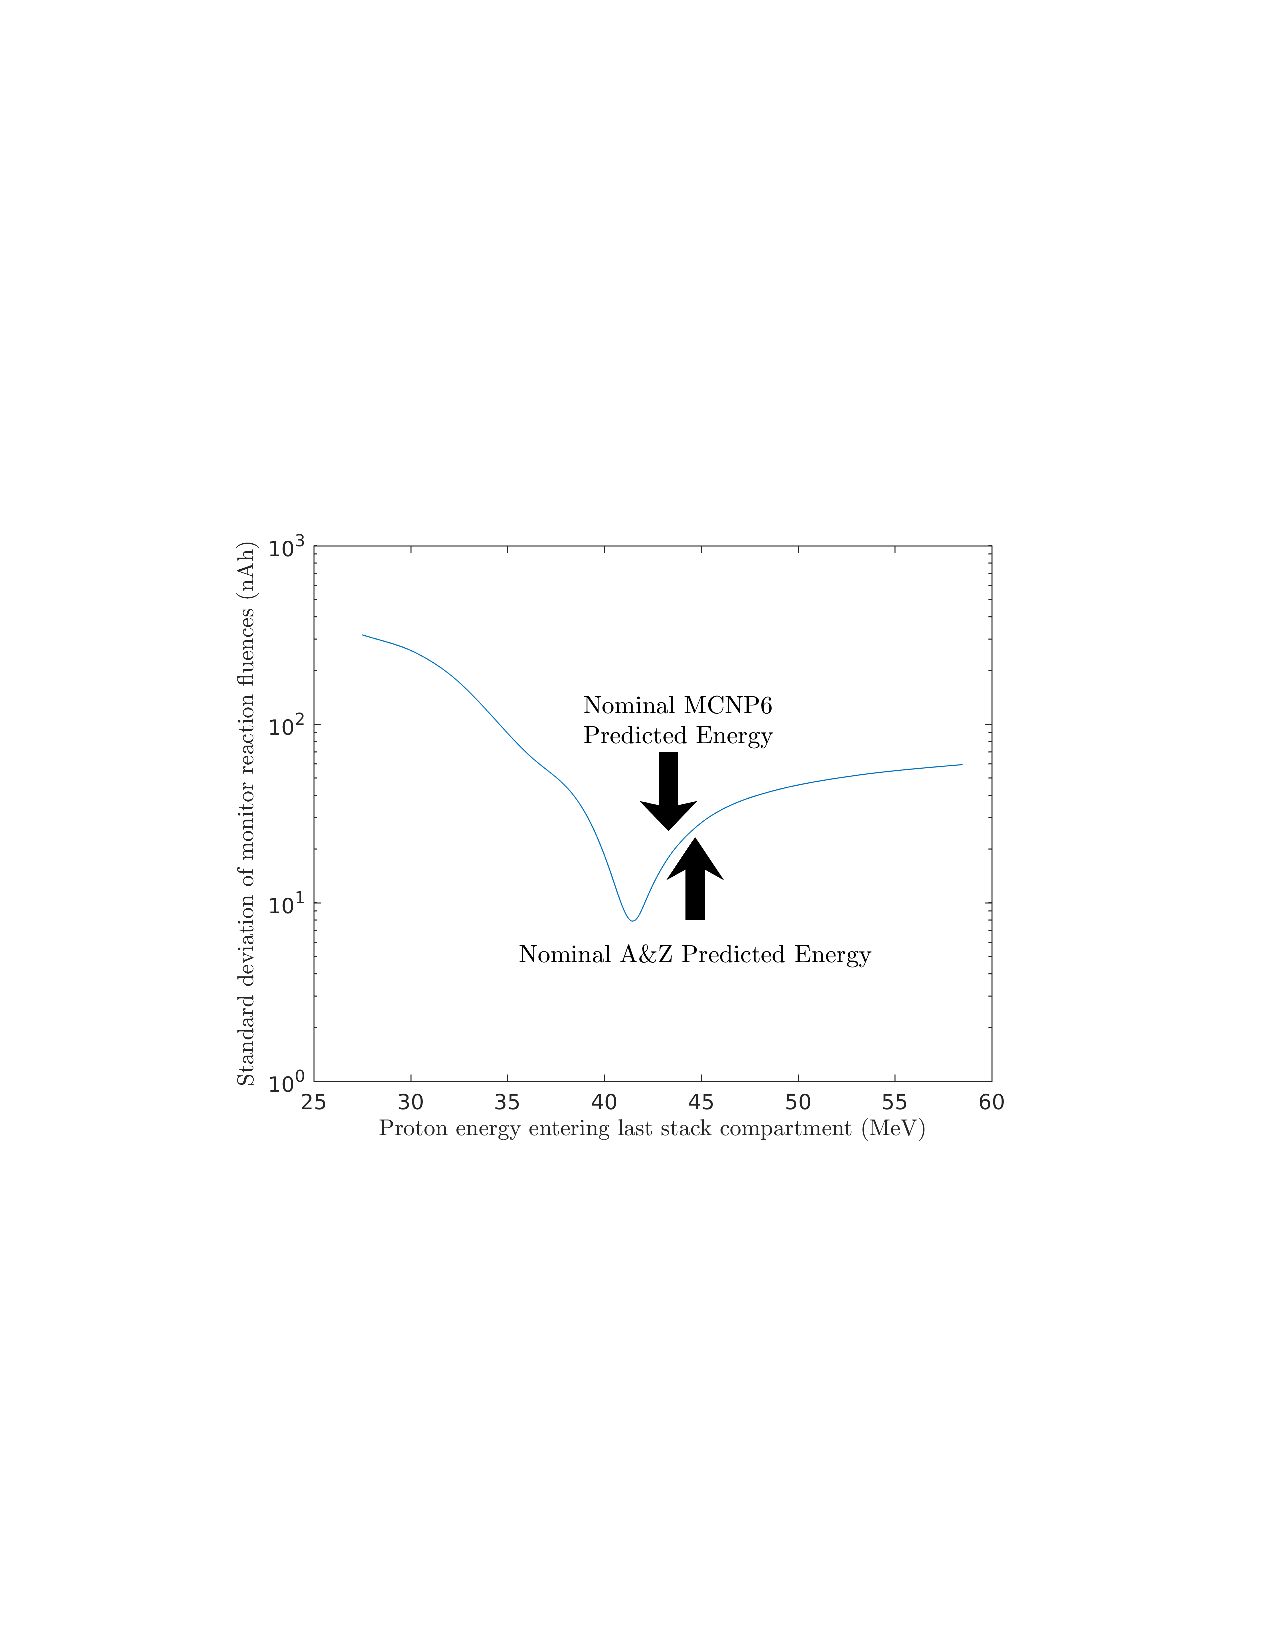
\includegraphics[clip=true,trim=1.5in 3.4in 1.8in 3.5in, scale=0.8]{./figures/variation_curve.pdf}
 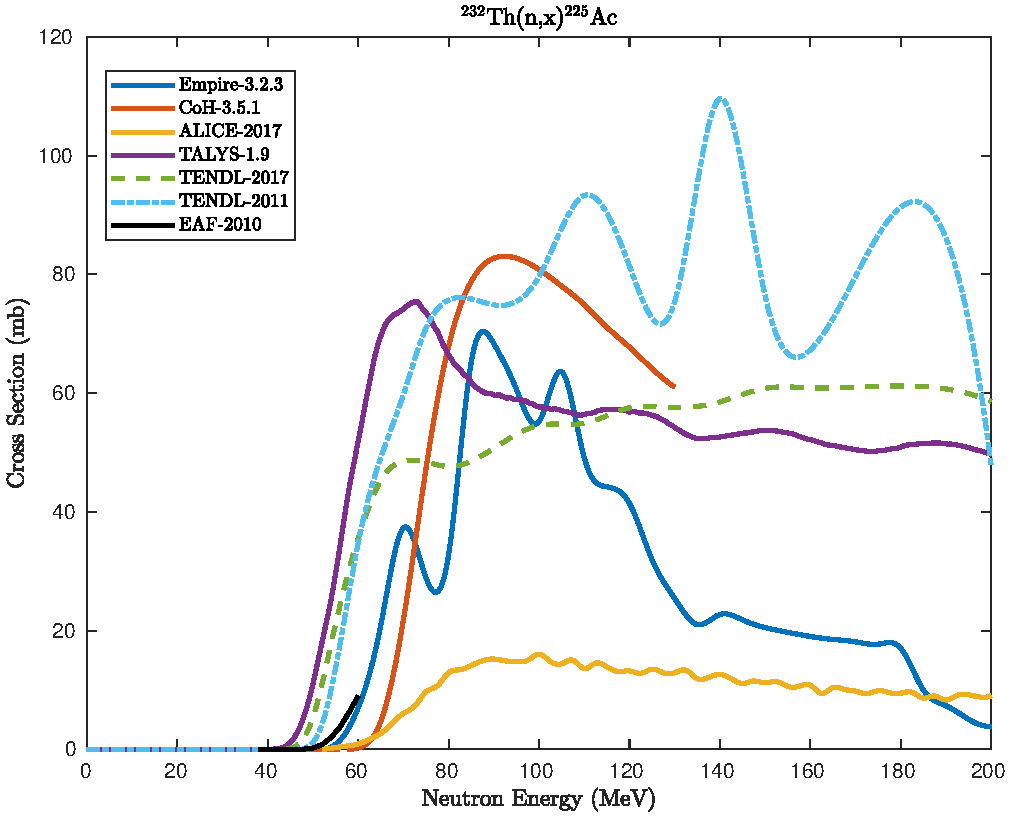
\includegraphics[width=0.7\linewidth]{225Ac.pdf}

 % variation_curve.pdf: 612x792 pixel, 72dpi, 21.59x27.94 cm, bb=0 0 612 792
 \caption{Predictions of several major reaction model codes for the (n,x) reactions leading to the production of \ce{^{225}Ac}.  Differences of up to an order of magnitude are commonly seen.    }
 \label{fig:ithemba_plot}
\end{figure}

Unfortunately, accurate modeling of these high-energy reactions is notoriously difficult.  \autoref{fig:ithemba_plot} shows a comparison between cross sections for the production of \ce{^{225}Ac} from (n,x) reactions on \ce{^{232}Th} calculated with the reaction codes typically used to predict isotope production.  This includes EMPIRE-3.2.3 \cite{Herman2013}, CoH 3.5.1 \cite{KAWANO2010}, ALICE-2017 \cite{Blann1996}, the TENDL-2011 and TENDL-2017 libraries produced using TALYS \cite{Rochman2017}, as well as the most recent version of the code (TALYS 1.9) \cite{Koning2012} and the European Activation File (EAF-2010) \cite{Forrest2005}.  Differences on the order of 50--100\% are often seen.  

These large uncertainties in reaction modeling means that direct measurement of the reaction cross sections themselves are needed in order to design targets capable of efficiently producing low-contamination radionuclides.  Fortunately, most of the reactions of interest take place on stable targets and are therefore experimentally accessible. 

The preferred method for measuring these cross sections involves foil activation, in which one or more well-characterized thin foil(s) is/are irradiated and the residual radioactivities are quantified through off-line alpha, beta, gamma, or electron spectroscopy \cite{Voyles2018a,Graves2016}.  The uncertainty in the deduced cross section depends strongly on the accurate characterization of the target material (which is often challenging to produce), the spectroscopic assaying techniques used and precise determination of the incident particle flux. Access to well-characterized nuclear data can be useful in reducing the first two sources of uncertainty. 


The flux is typically determined using a well-characterized monitor reaction on a co-irradiated foil that leads to the production of an easily quantified, long-lived residual nucleus. However, for both charged-particle and neutron-induced reactions, there relatively few monitor reactions that can be applied in the low- to intermediate-energy regimes of 30--70 MeV.  The situation is worse above 70 MeV, where monitor reactions  free from the potential influence of secondary neutron contributions are even harder to come by.  Knowledge of these cross sections as a function of the incident particle energy is essential to  isotope production, with recent efforts focused on developing  \ce{^{93}Nb}(p,4n)\ce{^{90}Mo} ($t_{1/2}$= 5.56(9) hours) as a monitor reaction reaction suitable for use at regional isotope production facilities \cite{Voyles2018a, Kim2018}.  


\section{NUCLEAR ENERGY}

Reliable modeling and simulation predictions of nuclear energy systems is essential to the design, licensing, and operation of nuclear power stations, as well as the fuel cycle facilities for enrichment and material processing, fuel fabrication, transportation and storage. Additional predictive calculations are required for spent fuel characterization for storage, transportation and disposal as well as hardware activation and radiation shielding and personnel protection. Nuclear data and their uncertainties are required for a wide range of calculations including:
\begin{itemize}
  \item Reactor core and fuel design,
  \item Safety parameter assessment,
  \item Criticality safety,
  \item Shielding,
  \item Material damage in structures,
  \item Decay heat at reactor shut-down,
  \item Decay heat in storage and transportation,
  \item Mass flow in the fuel cycle, and
  \item Material safeguards.
\end{itemize}

The nuclear physics of these systems are inferred from (n,x) cross sections, fission spectra, neutron multiplicity, fission product yields, decay constants, branching ratios, gamma yields, delayed neutron precursors, and more.  For light water reactors (LWRs), nuclear data have been used, tested, and often \enquote{tuned}, over many decades to provide acceptable results, and there is an abundance of documented benchmark quality experiments and plant operation data for the validation of common scenarios. However, for new applications such as fuels and materials in advanced reactors, accident tolerant fuels, high burnup fuel, and spent fuel repository scenarios, there are many needs to improve nuclear data and assess the availability of benchmark experiments that could be applied for testing and validation. 

One artifact of the nuclear data tuning process is a reduction in confidence due to compensating errors. Where fission and capture reactions are modified to ensure that the integral value of $k_{eff}$ is maintained, little confidence remains in the independent use of the fission cross section itself, which is essential to the prediction of reactor power distributions. These power distributions are essential to the prediction of peak fuel temperatures during a reactor transient to ensure that the fuel does not exceed thermal limits that are set to ensure fuel integrity. Reduced confidence in the fission cross section can have real consequences in the allowed power level and operating regimes for these systems.

In a study conducted by SG46, it was found that many individual reactions were modified by several percent from ENDF/B-VII.1 to ENDF/B-VIII.0 with some examples shown in \autoref{fig:ne_plots}.



\begin{figure}
    \centering
    \begin{minipage}{0.5\textwidth}
        \centering
        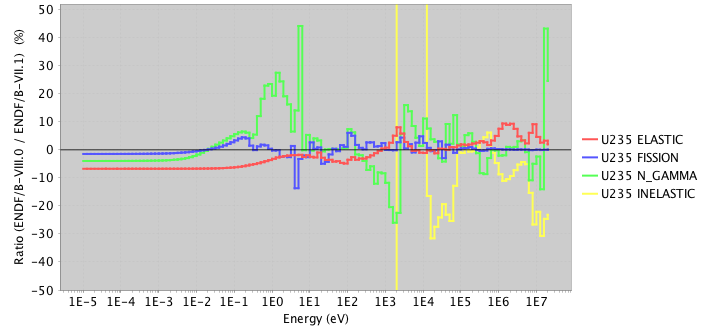
\includegraphics[width=0.97\textwidth]{u235.png} % first figure itself
%         \caption{first figure}
    \end{minipage}\hfill
    \begin{minipage}{0.5\textwidth}
        \centering
        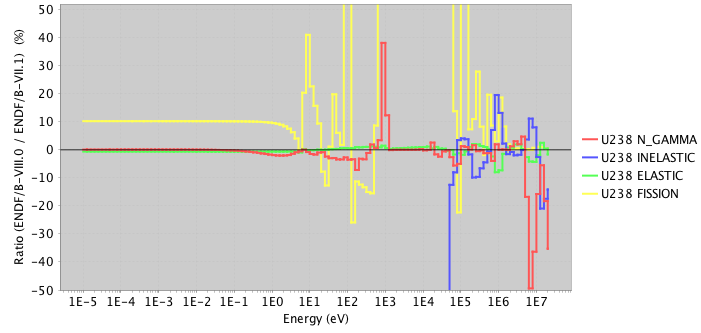
\includegraphics[width=0.97\textwidth]{u238.png} % second figure itself
%         \caption{second figure}
    \end{minipage}
    \\
    \centering
    \begin{minipage}{0.5\textwidth}
        \centering
        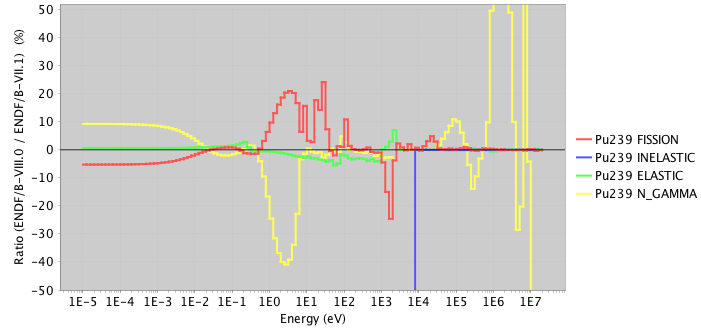
\includegraphics[width=0.97\textwidth]{pu239_1.png} % first figure itself
%         \caption{first figure}
    \end{minipage}\hfill
    \begin{minipage}{0.5\textwidth}
        \centering
        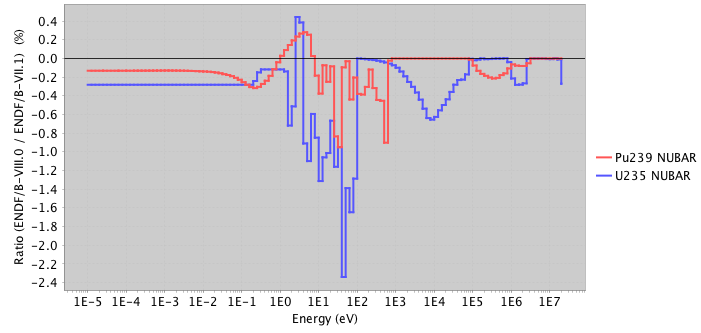
\includegraphics[width=0.97\textwidth]{pu239_2.png} % second figure itself
%         \caption{second figure}
    \end{minipage}
    \caption{SG46 findings on changes in cross sections from ENDF/B-VII.1 to ENDF/B-VIII.0 of key nuclides. }
     \label{fig:ne_plots}
\end{figure}

% \begin{figure}
%     \centering
% %     \subfloat{
%         \centering
% %         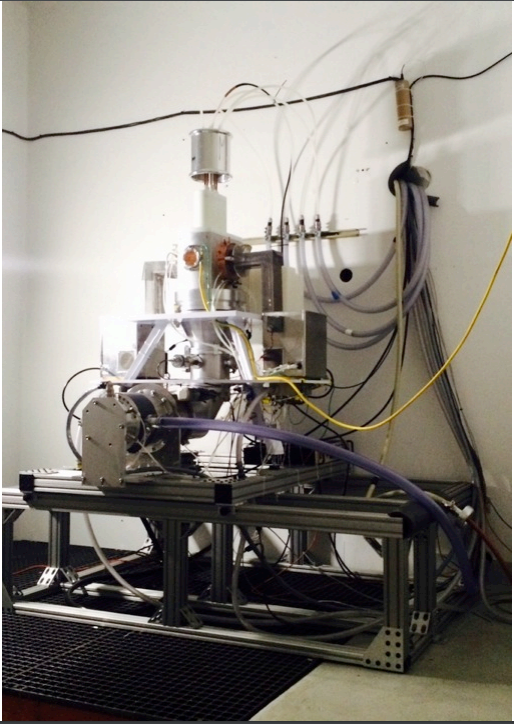
\includegraphics[width=\columnwidth]{./figures/Capture.PNG}
%         \hspace{-5pt}\subfigimg[width=0.5\textwidth]{}{u235.png}{50}
% %         \caption{ Decay curve for the isomeric transition of \ce{^{115m}In}.}
%          %         \refstepcounter{subfigure}
% %          \label{fig:before_minimization}
%    \hspace{-5pt}%
% %      \subfloat{
%         \centering
% %         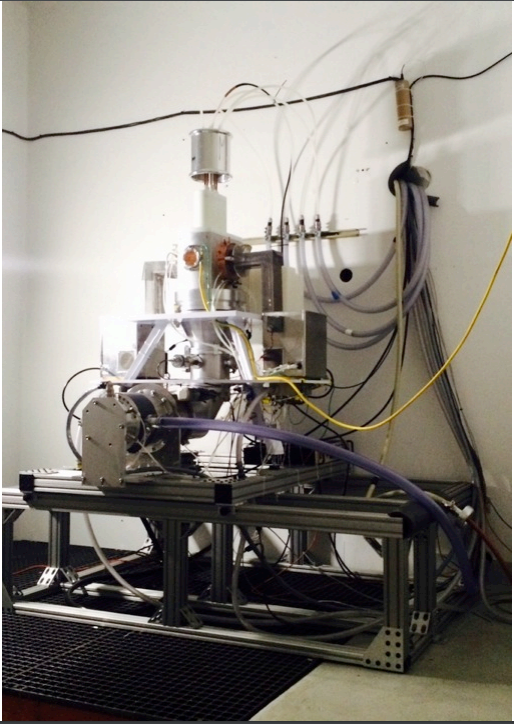
\includegraphics[width=\columnwidth]{./figures/Capture.PNG}
% %         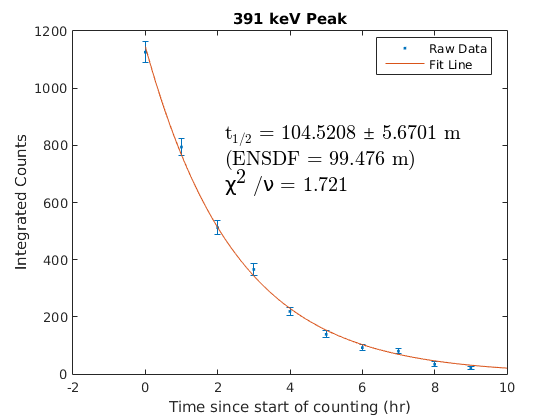
\includegraphics[scale=0.6]{./figures/391keV_curve2.png}
%         \subfigimg[width=0.5\textwidth]{}{u238.png}{50}
% %         \caption{ Decay curve for the isomeric transition of \ce{^{113m}In}.}
%          %         \refstepcounter{subfigure}
% %          \label{fig:after_minimization}
%    \hspace{-5pt}%\\
%        \centering
% %     \subfloat{
%         \centering
% %         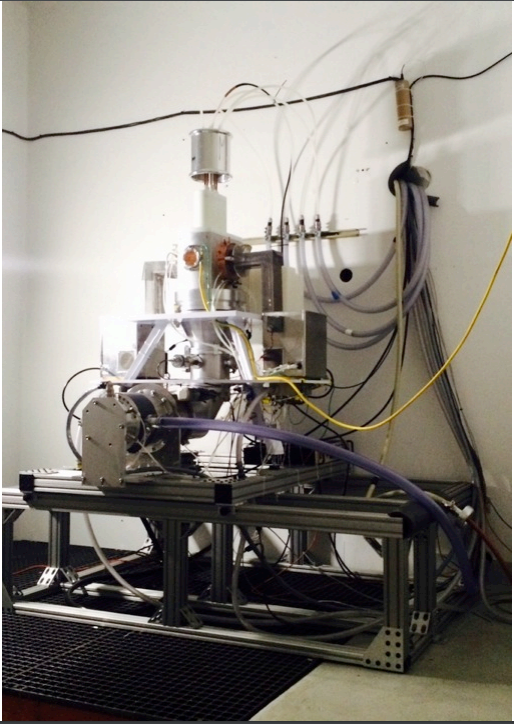
\includegraphics[width=\columnwidth]{./figures/Capture.PNG}
%         \hspace{-5pt}\subfigimg[width=0.5\textwidth]{}{pu239_1.png}{50}
% %         \caption{ Decay curve for the isomeric transition of \ce{^{115m}In}.}
%          %         \refstepcounter{subfigure}
% %          \label{fig:before_minimization}
%    \hspace{-5pt}%
% %      \subfloat{
%         \centering
% %         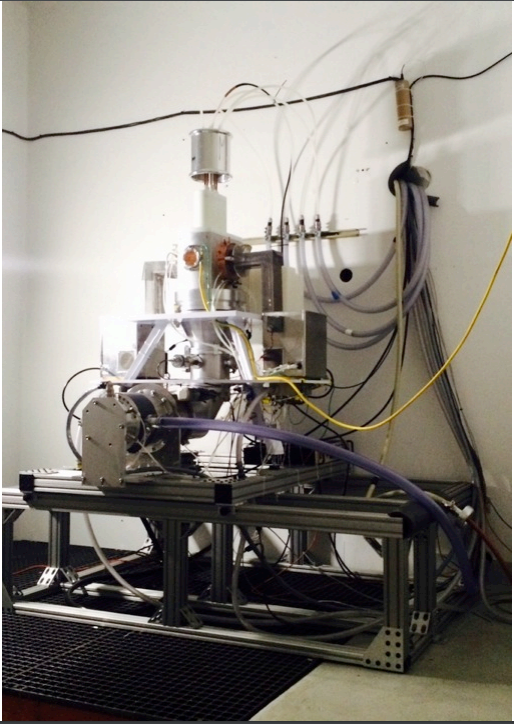
\includegraphics[width=\columnwidth]{./figures/Capture.PNG}
% %         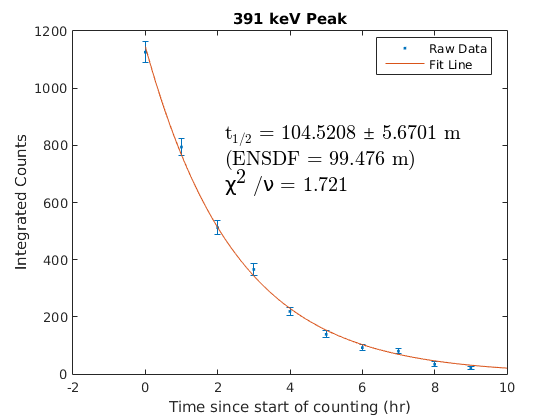
\includegraphics[scale=0.6]{./figures/391keV_curve2.png}
%         \subfigimg[width=0.5\textwidth]{}{pu239_2.png}{50}
% %         \caption{ Decay curve for the isomeric transition of \ce{^{113m}In}.}
%          %         \refstepcounter{subfigure}
% %          \label{fig:after_minimization}
%    \hspace{-5pt}%
%     \caption{SG46 findings on changes in cross sections from ENDF/B-VII.1 to ENDF/B-VIII.0 of key nuclides. }
%      \label{fig:ne_plots}
% \end{figure}

Many of these advanced systems also require so-called high-assay low enriched uranium (HA-LEU), which has a \ce{^{235}U} enrichment \textgreater5\% and \textless20\% by mass, where the current fleet of LWRs utilize enrichments of 5\% or less. With few benchmark experiments in HA-LEU enrichment range, the interplay of the cross sections for multiple nuclei become important, especially for LEU experiments where \ce{^{1}H}, \ce{^{16}O}, \ce{^{235}U}, \ce{^{238}U} and others are applied simultaneously in the calculation of the integral $k_{eff}$ response.  Similar to the Chadwick \cite{Cha18} and Bauge \cite{Bau12} studies of Jezebel critical assembly, a team at ORNL preformed an investigation of a hypothetical transportation package with 20\% enriched \ce{^{235}U} in the form of \ce{UF6} using ENDF/B-VII.1 and ENDF/B-VIII.0 libraries by only exchanging the CIELO nuclides. A swing in $k_{eff}$ of 450 pcm is observed.  Future investigation and validation are required to gain confidence in either calculation.

Many nuclear data needs have been identified that are important for design and operating analysis for these advanced systems including:
\begin{itemize}
  \item Improving our knowledge of the \ce{^{238}U}(n,n')cross section.   \ce{^{238}U}(n,n') is a limiting factor in the design of fast spectrum reactors such as those with metallic cores or chloride salts. The 40\% uncertainty in this cross section in ENDF/B-VII.1 propagates to an uncertainty of 1.5\%$\Delta k$ in the criticality state of a sodium fast reactor (i.e. at the 2$\sigma$ level, $k_{eff}$ could range from 0.97 to 1.03 based on this uncertainty prediction) \cite{touran2016sensitivities}.
  \item Improved knowledge of the \ce{^{35}Cl}(n,p) cross section.  Changes from the 2006 release of ENDF/B-VII.0 to the 2011 release of ENDF/B-VII.1 are causing a 2-3\%$\Delta k$ change in reactivity in molten salt reactors. This data change will also impact repository analysis in salts and there are no benchmark experiments available for validation. Recent results from activation using a DD-neutron source \cite{voy18a} indicate both resonant behavior in this cross section and an average value significantly smaller value for  $2.2 < E_n (MeV) < 2.7$ \cite{Bat18].  
  \item Graphite data for high-temperature reactors as well as the Transient Reactor Test Facility (TREAT) facility have realized a number of updates that cause dramatic changes in criticality. Updates from ENDF/B-VII.0 to ENDF/B-VII.1 lead to a 1\%$\Delta k$ change in reactivity for the High Temperature Engineering Test Reactor (HTTR), leading to the calculations better matching experimental values. Proposed updates to the graphite thermal scattering data for the ENDF/B-VIII.0 release have been demonstrated to cause a 2\%$\Delta k$ change in reactivity for the TREAT M8CAL benchmark \cite{hawarithermal}.
  \item Thermal neutron scattering in molten salts, such as FLiBe. There are no cross-section data that represent the effect of the molecular bonds, leading to a computational bias of unknown magnitude in all reactor design calculations. The molecular bonds in water vs. Polyethylene can lead to a computation bias of 1-2\%$\Delta k$.  In addition, this effect is temperature dependent and is not well studied or understood. A recently developed benchmark experiment evaluation of the Molten Salt Reactor Experiment which consisted of uranium fuel FLiBe molten salt flowing through graphite channels demonstrates a bias of over 1\%$\Delta k$ from the experimental value \cite{shenzero}, with other presented results showing biases over 3\%$\Delta k$
  \item (n,x) reactions on heavy actinides that will buildup in molten salt reactors and high burnup fuel are poorly quantified and benchmark data are rare, so these effects are almost completely unknown.
  \item Uncertainties provided with ENDF in the form of cross section covariance data are often not mature and may or may not represent the true uncertainty in the nuclear data. For the recent ENDF/B-VIII.0 release, the readme file provided by the National Nuclear Data Center (NNDC) provides a disclaimer warning against the use of covariance data without applying a sensitivity/uncertainty approach to adjust the uncertainties for application specific analysis using relevant benchmark experiments. This specialized process is generally not available to users and presents many complicated aspects even for experts in the field, leaving a large gap between data provided by nuclear data evaluators and those useful for application in safety and design calculations.
  \item Nuclear data are gathered from many different sources, not only ENDF but also the ENSDF as well as the Joint European Fission Fusion (JEFF) library, which often have differing representations of the same data. The process of sorting through the data to correct inconsistencies and benchmark the consolidated library against benchmark experiments is complex.
  \item Uncertainty data are not available or are incomplete for fission product yields, decay constants, and angular distributions, making it difficult to have high confidence in predicting the performance of advanced systems.
\end{itemize}



The generation and distribution of nuclear data as well as the benchmarking of the performance of codes and data is a global effort. In the US, nuclear data are generated by teams supported by DOE-NP and NNSA. These teams gather at the Cross Section Evaluation Working Group meetings to create and test the ENDF libraries prior to distribution. They advocate for improved performance for their own applications, but because nuclear energy interests are not well represented at the review meetings, the impact of updates to nuclear data and associated uncertainty information on nuclear energy applications is often overlooked.

\section{FUTURE DIRECTIONS IN NUCLEAR DATA}

In recent years there has been a growing recognition of the need to develop a plan that addresses nuclear data needs from measurement through, compilation and evaluation in an organized, multi-agency fashion.  This process started in July 2014 with the first review of the US Nuclear Data Program, which is administered through the Nuclear Physics office in the US Department of Energy (DOE-NP), in nearly two decades.  The review stated that experimental efforts to address gaps in nuclear data are within the scope of the USNDP program, resulting in  DOE-NP requesting that a Nuclear Data Needs and Capabilities for Applications Workshop (NDNCA) be organized to compile a listing of nuclear data needed for nuclear energy, national security and isotope production.  NDNCA was held in Berkeley in May 2015  and a whitepaper delineating these needs was released 5 months later \cite{bernstein2015nuclear}.   The whitepaper provides a long and comprehensive list of nuclear data needs, both cross-cutting and application specific, that has served as the basis for multiple subsequent roadmapping efforts.

Following NDNCA, Dr. Catherine Romano, working with the DOE-NP and the NNSA office on counter-proliferation research and development (NA-22), organized a grassroots \enquote{Nuclear Data Working Group} (NDWG) comprised of subject matter experts selected by program managers from DOE-NP, DOE-Nuclear Energy, the Isotopes Program, the Department of Homeland Security and the several offices within the National Nuclear Security Administration to identify a \enquote{roadmap} to address the most important and crosscutting nuclear data needs including all steps in the nuclear data pipeline from measurement through compilation, evaluation and processing.  The NDWG presented their results to participating program managers as well as other interested agencies during the Nuclear Data Exchange Meeting (NDEM) in April 2016.  The scope of the recommended work included:
\begin{enumerate}
  \item infrastructure modernization, 
  \item expanded covariance data, 
  \item inelastic scatter on \ce{^{235}U}, \ce{^{238}U} and 239Pu, 
  \item gamma emission data, 
  \item fission yields, and 
  \item renewed nuclear data target production capabilities.
\end{enumerate}  
The NDEM provided a venue for valuable discussions between the nuclear data community and program managers and the tasks required to provide evaluated nuclear data to the database.  

In response to the plan presented by the NDWG, the program managers formed their own Nuclear Data Inter-Agency Working Group (NDIAWG) to pursue a collaborative effort to address several of these high-profile nuclear data needs in a cooperative fashion.  The NDIAWG issued two Funding Opportunity Announcements in 2017 and 2018 that led to a total of 11 new projects covering topics from improving fission fragment yield and gamma-ray decay data to measuring specific high-priority cross sections for isotope production and neutron transport for nuclear reactors.   

A key element of the NDIAWG process is ensuring that the efforts to address these nuclear data needs result in user impact.  This is accomplished by reviewing the progress made via recurring interagency workshops.  These workshops initially served as roadmapping discussions where the nuclear data users explained their needs, and the nuclear data community agreed upon a best path forward.  Now that several projects are underway, the workshops also serve as a project review. The first of these was the Nuclear Data Roadmapping Enhancement Workshop (NDREW) held in Washington DC in January 2018, which focused on nuclear data needs relevant to non-proliferation \cite{Ndr18} and resulted in a nuclear data roadmap for NNSA, DNN R\&D.  The second of these, a Workshop on Applied Nuclear Data Activities (WANDA) is planned for January 2019 in Washington DC and will cover topics relevant to nuclear energy, isotope production, safeguards and the medical community.  

The NDIAWG process reflects a growing recognition that improved nuclear data is essential to a wide range of human endeavors that transcend the needs of any one societal need or governmental mission.  Its goal is the development of a new, multi-agency national plan to address nuclear data needs in a coherent way.  This plan, which is being developed in partnership with international collaborators at the IAEA and the OECD-NEA represents a new paradigm for collaborative research.  

\section{CONCLUSION \texorpdfstring{---}{-} RETAINING AND TRAINING A SKILLED NUCLEAR DATA WORKFORCE}

A robust nuclear data evaluation process is needed to provide the information required for many applications ranging from nonproliferation to nuclear energy to isotope production.  However, it takes many years of post-Ph.D. experience to train nuclear data evaluators, and only a short break in support to lose  this work force to other pursuits.  It is therefore critical for the many societal programs that rely on nuclear data to support individuals engaged in maintaining all functions that make up the \enquote{Nuclear Data Pipeline}, from measuring and modeling through compilation, evaluation, validation, and processing.  As more and more of the research in the United States moves over to a project-driven model, it is imperative that sponsors coordinate their efforts to ensure that there is no loss of talent in the field.  The NDIAWG discussed above is a significant step to help address these issues in a systematic fashion.

Furthermore, nuclear data evaluation is an \emph{aging} field, with the mean age of an evaluator in the US being well-over 50.  It is essential that the next generation of nuclear data evaluators be recruited and trained while the current set of experienced individuals are still active in the field.  This is particularly challenging since there is, \emph{per se}, no graduate education program in nuclear data evaluation, and the vast majority of the centers with evaluation expertise are not associated with degree-granting institutions.  

Perhaps one of the \enquote{endangered species} in nuclear data is the experimental nuclear data evaluator.  This isn't an experimentalist doing a new, better experiment, nor a data library creator that makes an ENDF-like library, but a person who knows which of the more than 22,000 measurements in the EXFOR/CSISRS library are to be taken seriously, discarded or normalized to newer standards.  This sort of a \enquote{hybrid} individual would be capable of providing not only good mean values, but also the well-quantified uncertainties (including covariances) that are needed for most applications.  A concerted effort on the part of both academia and the international research community is needed to ensure that talented early-career individuals with the right combination of interest and inclination be afforded the opportunity to get trained by an \enquote{international village} of evaluators and application subject matter experts.  

In closing, it is worth noting that the dramatic increase in computational capabilities over the past several decades allows for the sort of detailed calculations needed to fulfill the promise of many applications, \emph{provided that the correct evaluated data is available}.   Recent efforts in the US offer the promise of a national nuclear data plan to provide the needed data.  If these efforts are maintained it could help herald in a world with a new sense of safety from enhanced nonproliferation capabilities, a new source of safe, carbon-neutral energy and a new class of radio-pharmaceuticals to diagnose and treat illness.  

% 
% %Heading 1
% \section{FIRST-LEVEL HEADING}
% This is dummy text. 
% % Heading 2
% \subsection{Second-Level Heading}
% This is dummy text. This is dummy text. This is dummy text. This is dummy text.
% 
% % Heading 3
% \subsubsection{Third-Level Heading}
% This is dummy text. This is dummy text. This is dummy text. This is dummy text. 
% 
% % Heading 4
% \paragraph{Fourth-Level Heading} Fourth-level headings are placed as part of the paragraph.

%Example of a Figure
% \section{ELEMENTS\ OF\ THE\ MANUSCRIPT} 
% \subsection{Figures}Figures should be cited in the main text in chronological order. This is dummy text with a citation to the first figure (\textbf{Figure \ref{fig1}}). Citations to \textbf{Figure \ref{fig1}} (and other figures) will be bold. 
% 
% \begin{figure}[h]
% 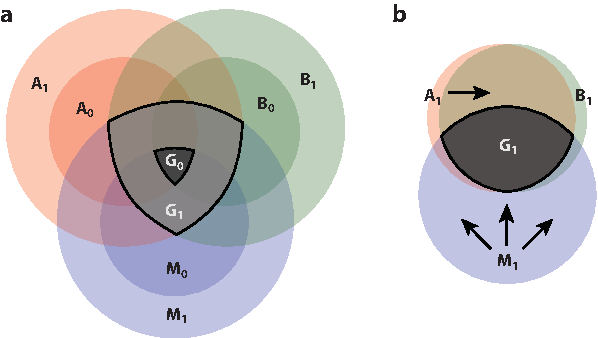
\includegraphics[width=3in]{SampleFigure.pdf}
% \caption{Figure caption with descriptions of parts a and b}
% \label{fig1}
% \end{figure}
% 
% % Example of a Table
% \subsection{Tables} Tables should also be cited in the main text in chronological order (\textbf {Table \ref{tab1}}).
% 
% \begin{table}[h]
% \tabcolsep7.5pt
% \caption{Table caption}
% \label{tab1}
% \begin{center}
% \begin{tabular}{@{}l|c|c|c|c@{}}
% \hline
% Head 1 &&&&Head 5\\
% {(}units)$^{\rm a}$ &Head 2 &Head 3 &Head 4 &{(}units)\\
% \hline
% Column 1 &Column 2 &Column3$^{\rm b}$ &Column4 &Column\\
% Column 1 &Column 2 &Column3 &Column4 &Column\\
% Column 1 &Column 2 &Column3 &Column4 &Column\\
% Column 1 &Column 2 &Column3 &Column4 &Column\\
% \hline
% \end{tabular}
% \end{center}
% \begin{tabnote}
% $^{\rm a}$Table footnote; $^{\rm b}$second table footnote.
% \end{tabnote}
% \end{table}
% 
% % Example of lists
% \subsection{Lists and Extracts} Here is an example of a numbered list:
% % \begin{enumerate}
% % \item List entry number 1,
% % \item List entry number 2,
% % \item List entry number 3,\item List entry number 4, and
% % \item List entry number 5.
% % \end{enumerate}
% 
% % Here is an example of a extract.
% % \begin{extract}
% % This is an example text of quote or extract.
% % This is an example text of quote or extract.
% % \end{extract}
% 
% \subsection{Sidebars and Margin Notes}
% % Margin Note
% \begin{marginnote}[]
% \entry{Term A}{definition}
% \entry{Term B}{definition}
% \entry{Term C}{defintion}
% \end{marginnote}
% 
% \begin{textbox}[h]\section{SIDEBARS}
% Sidebar text goes here.
% \subsection{Sidebar Second-Level Heading}
% More text goes here.\subsubsection{Sidebar third-level heading}
% Text goes here.\end{textbox}
% 
% 
% 
% \subsection{Equations}
% % Example of a single-line equation
% \begin{equation}
% a = b \ {\rm ((Single\ Equation\ Numbered))}
% \end{equation}
% %Example of multiple-line equation
% Equations can also be multiple lines as shown in Equations 2 and 3.
% \begin{eqnarray}
% c = 0 \ {\rm ((Multiple\  Lines, \ Numbered))}\\
% ac = 0 \ {\rm ((Multiple \ Lines, \ Numbered))}
% \end{eqnarray}
% 
% % Summary Points
% \begin{summary}[SUMMARY POINTS]
% \begin{enumerate}
% \item Summary point 1. These should be full sentences.
% \item Summary point 2. These should be full sentences.
% \item Summary point 3. These should be full sentences.
% \item Summary point 4. These should be full sentences.
% \end{enumerate}
% \end{summary}
% 
% % Future Issues
% \begin{issues}[FUTURE ISSUES]
% \begin{enumerate}
% \item Future issue 1. These should be full sentences.
% \item Future issue 2. These should be full sentences.
% \item Future issue 3. These should be full sentences.
% \item Future issue 4. These should be full sentences.
% \end{enumerate}
% \end{issues}

%Disclosure
\section*{DISCLOSURE STATEMENT}
\textred{IThe authors are not aware of any affiliations, memberships, funding, or financial holdings that might be perceived as affecting the objectivity of this review. }

% Acknowledgements
\section*{ACKNOWLEDGMENTS}
Work at Brookhaven National Laboratory was sponsored by the Office of Nuclear Physics, Office of Science of the U.S. Department of Energy under Contract \# DE-AC02-98CH10886 with Brookhaven Science Associates, LLC.

The authors acknowledge support for this work from the United States Department of Energy, Office of Science via the Isotope Development and Production for Research and Applications subprogram in the Office of Nuclear Physics. 

Work at Lawrence Berkeley National Laboratory has been carried out  under the auspices of the U.S. Department of Energy by  Lawrence Berkeley National Laboratory and the U.S. Nuclear Data Program under contract \# DE-AC02-05CH11231. This work used the Savio computational cluster resource provided by the Berkeley Research Computing program at the University of California, Berkeley (supported by the UC Berkeley Chancellor, Vice Chancellor for Research, and Chief Information Officer).

\textred{EVERYONE - Please provide me snippets of any other Acknowledgements you want included!}

% References
%
% Margin notes within bibliography
\section*{LITERATURE\ CITED}

\emergencystretch=2em


\bibliographystyle{ar-style5}

\bibliography{../../library}




 

% \end{thebibliography}


\end{document}
